\documentclass{article}
\usepackage{graphicx} % Required for inserting images
\usepackage{amsmath}
\usepackage{amssymb}
\usepackage{mathrsfs}
\usepackage[margin=0.5in]{geometry}
\usepackage{multicol}
\usepackage{hyperref}
\usepackage{cancel}
\usepackage{pgfplots}
\usepackage{changepage}
\usepackage{pgfplots}
\usepackage{amsthm}
\usepackage{tikz}
\usepackage{framed}
\usepackage{array}

\usepackage [english]{babel}
\usepackage [autostyle, english = american]{csquotes}
\MakeOuterQuote{"}

\usepackage[shortlabels]{enumitem}

\setlength{\parskip}{\baselineskip}%
\setlength{\parindent}{0pt}%

\newcommand{\laplace}[1]{\mathscr{L}\left\{#1\right\}}
\newcommand{\laplaceinv}[1]{\mathscr{L}^{-1}\left\{#1\right\}}
\newcommand{\pd}[2]{\frac{\partial #1}{\partial #2}}
\newcommand{\gvec}[1]{\overrightarrow{#1}}
\newcommand{\magnitude}[1]{\left\lvert\left\lvert#1\right\rvert\right\rvert}

\pgfplotsset{compat=1.18}

\newtheorem{theorem}{Theorem}[section]
\newtheorem{theorem*}{Theorem}
\newtheorem{prop}{Proposition}[section]

\renewcommand{\qedsymbol}{$\blacksquare$}

\begin{document}

\definecolor{shadecolor}{gray}{0.9}

\setlength{\columnsep}{0.1in}

\begin{center}\section*{References}\end{center}

\begin{multicols*}{2}[]

\textbf{Thermodynamics}

Ideal Gas Relationships
\vspace{-1em}
\begin{enumerate}
\item[] Ideal Gas Law \[PV=mRT \]\[ Pv = RT\]\[PV = nR_u T\]
\item[] Compressibility Factor \[Pv = ZRT\]
\item[] Internal Energy of Ideal Gas \[\Delta u = \int_{T_1}^{T_2} c_v(T)dT \approx c_{v,avg}\Delta T\]
\item[] Enthalpy of Ideal Gas \[\Delta h = \int_{T_1}^{T_2} c_p(T)dT \approx c_{p,avg}\Delta T\]
\item[] Entropy of Ideal Gas \[\Delta S_\text{ideal gas} = \underbrace{c_v \ln (T_2 / T_1) + R\ln (V_2 / V_1)}_{c_v\text{ at average temperature}}\]
\[=\underbrace{c_p\ln (T_2 / T_1) - R\ln (P_2 / P_1)}_{c_p\text{ at average temperature}}\]
\end{enumerate}
\vspace{-1em}
Isentropic Ideal Gas Relationships
\vspace{-1em}
\begin{enumerate}
\item[]\[\left(\frac{T_2}{T_1}\right)_{s=\text{const}} = \left(\frac{v_1}{v_2}\right)^{k-1}\]

\item[]\[\left(\frac{T_2}{T_1}\right)_{s=\text{const}} = \left(\frac{P_2}{P_1}\right)^{(k-1)/k}\]

\item[]\[\left(\frac{P_2}{P_1}\right)_{s=\text{const}} = \left(\frac{v_1}{v_2}\right)^{k}\]
\end{enumerate}
\vspace{-1em}
Energy Balances
\vspace{-1em}
\begin{enumerate}
\item[] Nozzle and Diffuser \[\dot m \left(h_1 + \frac{v_1^2}{2}\right) = \dot m \left(h_2 + \frac{v_2^2}{2}\right)\]
\item[] Compressor \[\dot m h_1 + W_\text{in} = \dot m h_2\]
\item[] Pump (liquids only) \[\dot m h_1 + V(P_2-P_1) = \dot m h_2\]
\item[] Turbine \[\dot m h_1 = \dot m h_2 + W_\text{out}\]
\end{enumerate}
Carnot Efficiency
\vspace{-1em}
\begin{enumerate}
\item[] Heat Engine \[\eta = \frac{T_H-T_L}{T_H}\]
\item[] Heat Pump Coefficient of Performance \[\text{COP}_\text{HP} = \frac{T_H}{T_H-T_L}\]
\item[] Refrigerator Coefficient of Performance \[\text{COP}_\text{R} = \frac{T_L}{T_H-T_L}\]
\end{enumerate}
\vspace{-1em}
Heat-Entropy Relationship
\vspace{-1em}
\begin{enumerate}
    \item[] \[\Delta S = \frac{Q}{T_0}\]
    \item[] \[Q = \int_{T_1}^{T_2} TdS\]
\end{enumerate}
\vspace{-1em}
Isentropic Efficiency
\vspace{-1em}
\begin{enumerate}
\item[] Turbine \[\eta = \frac{W_a}{W_s} = \frac{h_1-h_{2a}}{h_1-h_{2s}}\]
\item[] Compressor \[\eta = \frac{W_s}{W_a} = \frac{h_{2s}-h_1}{h_{2a}-h_1} = \underbrace{\frac{V(P_2-P_1)}{h_{2a}-h_1}}_\text{Pumps}\]
\end{enumerate}
\vspace{-1em}
Cycle Efficiency
\vspace{-1em}
\begin{enumerate}
\item[] Otto Cycle \[\eta = 1 - \frac{1}{r^{k-1}}\]
\item[] Diesel Cycle \[\eta = 1 - \frac{1}{r^{k-1}}\left[\frac{r_c^k - 1}{k(r_c-1)}\right]\]
\item[] Brayton Cycle \[\eta = 1 - \frac{1}{r_p^{(k-1)/k}}\]
\item[] Rankine Cycle \[\eta = 1 - \frac{Q_\text{out}}{Q_\text{in}}\]
\item[] Backwork Ratio \[\text{BWR} = \frac{W_\text{in}}{W_\text{out}}\]
\end{enumerate}
\end{multicols*}

\begin{multicols*}{2}[]
\textbf{Statics and Mechanics of Materials}

\vspace{-0.5em}
Stress
\vspace{-0.5em}
\begin{enumerate}
        \item[] Normal Stress \[\sigma_{zz} = \frac{N}{A} + \frac{M_xy}{I_x} - \frac{M_yx}{I_y}\]
        \item[] Shear Stress (average) \[\tau_{zx} = \frac{V_x}{A},\ \tau_{zy} = \frac{V_y}{A}\]
        \item[] Shear Stress due to Torsion \[\tau_{z\theta} = \frac{Tr}{J}\]
\end{enumerate}
\vspace{-0.5em}
Strain
\vspace{-0.5em}
\begin{enumerate}
    \item[] Extensional Strain \[\epsilon = \frac{\sigma}{E} = \frac{\delta}{L_0} \]
    \item[] Shear Strain \[\gamma = \frac{\tau}{G} = \phi_1 + \phi_2\]
    \item[] Multiaxial Hooke's Law 
        \[\epsilon_x = \frac{\sigma_x}{E} - \frac{\nu\sigma_y}{E} - \frac{\nu \sigma_z}{E} + \alpha\Delta T\]
        \[\epsilon_y = \frac{\sigma_y}{E} - \frac{\nu\sigma_x}{E} - \frac{\nu \sigma_z}{E} + \alpha\Delta T\]
        \[\epsilon_z = \frac{\sigma_z}{E} - \frac{\nu\sigma_x}{E} - \frac{\nu \sigma_y}{E} + \alpha\Delta T\]
    \item[] Poisson's Ratio \[E = 2G(1+\nu)\]
\end{enumerate}
\vspace{0.5em}
Extension
\vspace{-0.5em}
\begin{enumerate}
    \item[] Normal Extension \[\delta = \frac{FL_0}{AE}\]
    \item[] Angle of Torsion \[\phi = \frac{TL}{JG}\]
\end{enumerate}
\vspace{-0.5em}
Centroid Locations
\vspace{-1em}
\begin{enumerate}
    \item[] \[A c_x = \sum A_i\overline{x}_i \iff c_x = \frac{\sum A_i\overline{x}_i}{A}\]
    \item[] \[A c_y = \sum A_i\overline{y}_i \iff c_y = \frac{\sum A_i\overline{y}_i}{A}\]
\end{enumerate}
\vspace{20.5em}
Area Moments of Inertia
\vspace{-0.5em}
\begin{enumerate}
    \item[] Parallel Axis Theorem \[I_{x'} = I_x +Ad^2\]
    \item[] Rectangular Section \[I = \frac{1}{12}bh^3\]
    \item[] Circular Section \[I_x = I_y = \frac{\pi r^4}{4} = \frac{\pi d^4}{64}\]
    \item[] Circular Section, Normal Axis \[J = \frac{\pi r^4}{2} = \frac{\pi d^4}{32}\]
\end{enumerate}
\vspace{-1em}
Principle Stress and Stress Transformations
\vspace{-1em}
\begin{enumerate}
    \item[] Stress Transformations \[\sigma_{x'} = \frac{\sigma_x + \sigma_y}{2}+ \frac{\sigma_x - \sigma_y}{2}\cos 2\theta + \tau_{xy}\sin2\theta\]
    \[\sigma_{y'} = \frac{\sigma_x + \sigma_y}{2} - \frac{\sigma_x - \sigma_y}{2}\cos 2\theta - \tau_{xy}\sin2\theta\]
    \[\tau_{x'y'} = -\frac{\sigma_x -\sigma_y}{2}\sin2\theta + \tau_{xy}\cos2\theta\]
    \item[] Principle Stresses \[\sigma_{1,2} = \frac{\sigma_x + \sigma_y}{2} \pm \underbrace{\sqrt{\left(\frac{\sigma_x - \sigma_y}{2}\right)^2 + \tau_{xy}^2}}_{\tau_{\text{max}}}\]
\end{enumerate}
\vspace{-1em}
Principle Strain and Strain Transformations
\vspace{-1em}
\begin{enumerate}
    \item[] Strain Transformations \[\epsilon_{x'} = \frac{\epsilon_x + \epsilon_y}{2} + \frac{\epsilon_x-\epsilon_y}{2}\cos(2\theta) + \frac{\gamma_{xy}}{2}\sin(2\theta)\]
    \[\epsilon_{y'} = \frac{\epsilon_x + \epsilon_y}{2} - \frac{\epsilon_x-\epsilon_y}{2}\cos(2\theta) - \frac{\gamma_{xy}}{2}\sin(2\theta)\]
    \[\frac{\gamma_{x'y'}}{2} = - \frac{\epsilon_x-\epsilon_y}{2}\sin(2\theta) + \frac{\gamma_{xy}}{2}\cos(2\theta)\]
    \item[] Principle Strains \[\epsilon_{1,2} = \frac{\epsilon_x+\epsilon_y}{2}\pm \underbrace{\sqrt{\left(\frac{\epsilon_x-\epsilon_y}{2}\right)^2 + \left(\frac{\gamma_{xy}}{2}\right)^2}}_{\gamma_{\text{max}}/2}\]
    \item[] Strain Gauge Rosette Relationship \[\epsilon_a = \epsilon_x\cos^2\theta_a + \epsilon_y \sin^2\theta_a + \gamma_{xy}\sin\theta_a\cos\theta_a\]
\end{enumerate}
\vspace{-1em}
Bending Deflections
\vspace{-1em}
\begin{enumerate}
    \item[] \[\frac{M}{EI} = \frac{d^2u}{dz^2} = \frac{d\theta}{dz}\]
\end{enumerate}
\end{multicols*}

\textbf{Dynamics and Vibrations}

\begin{multicols*}{2}[]
\vspace{-2em}
Rectilinear Motion
\vspace{-2em}
\begin{enumerate}
    \item[] \[a = v\frac{dv}{ds} \iff ads = vdv\]
\end{enumerate}
\vspace{-1em}
Coordinate Systems
\vspace{-1em}
\begin{enumerate}
    \item[] Polar Coordinates
\vspace{-1em}
    \[\vec{r} = r\hat e_r + z\hat k\]
\vspace{-1em}
    \[\vec{v} = \dot r\hat e_r + r\dot\theta \hat e_\theta + \dot z\hat k\]
\vspace{-1em}
    \[\vec{a} = (\ddot r - r\dot\theta^2)\hat e_r + (r\ddot\theta + 2\dot r\dot\theta)\hat e_\theta + \ddot z\hat k\]
\vspace{-1em}
    \item[] Normal-Tangential Coordinates
\vspace{-1em}
    \[\vec{v} = v\hat e_t\]
\vspace{-1em}
    \[\vec{a} = \dot v\hat e_t + \frac{v^2}{\rho}\hat e_n\]
\end{enumerate}
\vspace{-1em}
Particle Kinetics
\vspace{-1em}
\begin{enumerate}
    \item[] Newton's 2nd Law \[\sum \vec{F} = m\vec{a_c}\]

    \item[] Work-Energy Theorem \[\underbrace{\int_{\vec{R}_1}^{\vec{R}_2} \vec{F}\cdot d\vec{R}}_\text{Work} = \underbrace{T_2-T_1}_\text{Kinetic energy}\]

    \item[] Work-Energy Theorem, Conservative Forces

    \[T_1+V_1+W_\text{nonconservative} = T_2 +V_2\]

    \item[] Impulse-Momentum Equation \[\int_{t_1}^{t_2}\vec{F}dt = m\vec{v}_2 - m\vec{v}_1\]

    \item[] Coefficient of Restitution, rectilinear speeds \[e:=\frac{v_B' - v_A'}{v_A-v_B}\]
\end{enumerate}

Particle Vibrations
\vspace{-1em}
\begin{enumerate}
    \item[] Undamped natural frequency, spring-mass system \[\omega_n = \sqrt\frac{k}{m}\]
    \item[] Equation of Motion, Undamped Vibrations \[\ddot x + \omega_n^2x = 0\]
    \item[] Solution, Undamped Vibrations \[x(t) = x_0\cos(\omega_n t)+ \frac{\dot x_0}{\omega_n}\sin(\omega_n t)\]
    \vspace{-2.5em}
    \item[] Damping ratio, spring-mass damper \[\zeta = \frac{c}{2m\omega_n}\]
    \item[] Damped frequency \[\omega_d = \omega_n\sqrt{1-\zeta^2}\]
    \item[] Equation of Motion, Damped Vibrations \[\ddot x + 2\zeta\omega_n \dot x + \omega_n^2x = 0\]
    \item[] Solution, Damped Vibrations \[x(t) = e^{-\zeta\omega_nt}\left(x_0\cos(\omega_d t)+\frac{\dot x_0+\zeta\omega_nx_0}{\omega_d}\sin(\omega_d t)\right)\]
    \item[] Time Constant ($t=4\tau \implies 98\%$ decay) \[\tau = \frac{1}{\zeta\omega_n}\]
\end{enumerate}

\vspace{-1em}
Planar Rigid Body Kinetics
\vspace{-1em}
\begin{enumerate}
    \item[] General Velocity for Rigid Body (or bodies, points $o$ and $p$) \[\vec{v}_p = \vec{v}_o + \vec{\omega_o}\times\vec{r}_{p/o} + \vec{v}_{p\text{,rel }o}\]
    \item[] General Acceleration for Rigid Body (or bodies, points $o$ and $p$) \[\vec{a}_p = \vec{a}_o + \vec{\alpha}\times\vec{r}_{p/o}+\vec\omega_o\times(\vec{\omega_o}\times\vec{r}_{p/o}) + 2\vec\omega_o \times \vec{v}_{p\text{,rel }o} + \vec{a}_{p\text{,rel }o}\]
    \item[] Parallel Axis Theorem (from center of mass $c$ to point $p$ at distance $d$) \[I_p = I_c + md^2\]
    \item[] Euler's Equation \[\sum M_p = I_p\dot{\vec{\omega}} + \vec{r}_{c/p}\times m\vec{a}_p\]
\end{enumerate}
\vspace{-1em}
Planar Rigid Body Vibrations
\vspace{-1em}
\begin{enumerate}
    \item[] Equation of Motion, Forced Vibrations (with cosine forcing term) \[\ddot x + \frac{c}{m}\dot x + \frac{k}{m}x = \frac{F_0}{m}\cos(\omega_t)\]
    \item[] Tuning Ratio \[\eta = \frac{\omega}{\omega_n}\text{, where }\eta\approx1 \text{ at resonance}\]
    \item[] Steady-State Amplitude of Response, Forced Vibrations \[X = \frac{F_0/k_\text{effective}}{\sqrt{(2\zeta\eta)^2+(1-\eta^2)^2}}\]
    \item[] Steady-State Amplitude of Response, Base Excitations \[X = x_0\sqrt{\frac{1+(2\zeta\eta)^2}{(2\zeta\eta)^2+(1-\eta^2)^2}}\]
\end{enumerate}
\end{multicols*}

\tableofcontents

%% header:

%
%\begin{center}
%    Notes from \textbf{SUBJECT ###: Course Title}
%
%    taught at University of Michigan, [FALL/WINTER] YEAR
%
%    using \textit{Textbook Title}, by Textbook Author(s)
%\end{center}
%
%


\section{Thermodynamics}

\begin{center}
    Notes from \textbf{MECHENG 235: Thermodynamics I}

    Taken at University of Michigan, Fall 2024

    using \textit{Thermodynamics: an Engineering Approach}, by Boles and Cengel
\end{center}

\subsection{Basic Concepts of Thermodynamics}

\textbf{Thermodynamics} is the study of energy and its interaction with matter. In particular, \textit{classical thermodynamics} is the study of energy and energy transfer at a macroscopic level. Thermodynamics is concerned with the \textbf{equilibrium states} of systems.

A system has properties which may be \textbf{extensive} (varying with system size, i.e. total volume and total momentum) or \textbf{intensive} (not variable with size, i.e. temperature and pressure). A system is in \textit{equilibrium} when there are no forces driving change to the system. This equilibrium may be \textit{thermal} (temperature is constant with time), \textit{mechanical} (pressure is constant with time), or \textit{chemical} (chemical composition does not progress with time, no net reaction). A system may be \textbf{closed}, with a control mass and potentially variable volume, or \textbf{open}, with a control volume and potentially variable mass. A system is \textbf{adiabatic} if no heat is transferred (i.e. the system is well-insulated, or system is the same temperature as surroundings).

\begin{shaded}
    \textbf{The State Postulate.} The state of a simple compressible system is completely specified by \textit{two independent intensive properties}.
\end{shaded}

Other intensive properties of a system include \textbf{internal energy} $u$, and \textbf{enthalpy} $h$. Enthalpy is defined in terms of internal energy: \[H = U + PV\hspace{0.5in}(kJ)\] and specific enthalpy is similarly defined by \[h = u + Pv\hspace{0.5in}(kJ/kg)\] Internal energy is usually used in evaluating closed systems, while enthalpy may be used in evaluating open (flowing) systems.

\begin{shaded}
    \textbf{Zeroth Law of Thermodynamics.} If two bodies are in thermal equilibrium with a third body, they are also in thermal equilibrium with each other. If the third body is a thermometer, then the two bodies are in thermal equilibrium if they have the same temperature.
\end{shaded}

\subsection{Energy and the First Law of Thermodynamics}

Energy exists in several forms. There is \textbf{macroscopic energy} (kinetic, potential), \textbf{microscopic energy} (related to molecular structure and activity) and \textbf{internal energy, $U$} (sum of microscopic energies). In general, energy exists in either \textbf{static} or \textbf{dynamic} form:
\begin{enumerate}
    \item \textbf{Static energy}: stored in the system (ex. energy in chemical bonds).
    \item \textbf{Dynamic energy}: recognized only as it crosses a boundary (ex. heat, the flow of energy due to temperature difference at the boundaries; work, force applied to move a boundary)
\end{enumerate}

The \textbf{First Law of Thermodynamics} is the conservation law for energy:

\begin{shaded}
    \textbf{First Law of Thermodynamics.} Energy is not created or destroyed during a process and may only change forms. \[\underbrace{E_{in} - E_{out}}_{\text{macroscopic}} = \underbrace{\Delta E_{system}}_{\text{microscopic}}.\]
    For a cycle ($\Delta E_{system} = 0)$, the first law reduces to \[Q_{net}-W_{net} = 0\]
\end{shaded}

\subsection{Properties of Pure Substances}

A \textbf{pure substance} is any substance with a fixed, uniform chemical composition. A pure substance may be comprised of one element (i.e. nitrogen gas) or more (i.e. water), or a mixture of several substances which is homogeneous (i.e. air). The \textbf{phase} of a substance is dependent on the average movement of its molecules (temperature). During a \textbf{phase change}, some portion of a sample of substance exists in either phase, depending on the properties of substance. 

During a phase change from the liquid state to the gaseous state, a pure substance may be in any of the following phases:
\begin{enumerate}
    \item \textbf{Compressed liquid}. The substance is a liquid which is not about to vaporize.
    \item \textbf{Saturated liquid}. The substance is liquid, but any increase in temperature or decrease in pressure will cause it to partially vaporize.
    \item \textbf{Saturated liquid-vapor mixture}. The substance is a mix of gas and liquid. Without change to pressure, the temperature of a saturated vapor is constant, with only the volume changing during the process.
    \item \textbf{Saturated vapor}. The substance is a gas, but any decrease in temperature or increase in pressure will cause it to partially condense.
    \item \textbf{Superheated vapor}. The substance is a gas which is not about to vaporize.
\end{enumerate}

Pressure and temperature are dependent on each other during phase change, so another intensive property (generally specific volume, $v$) is required to describe the system. Plotting temperature or pressure against specific volume during a phase change gives the following:

\begin{center}
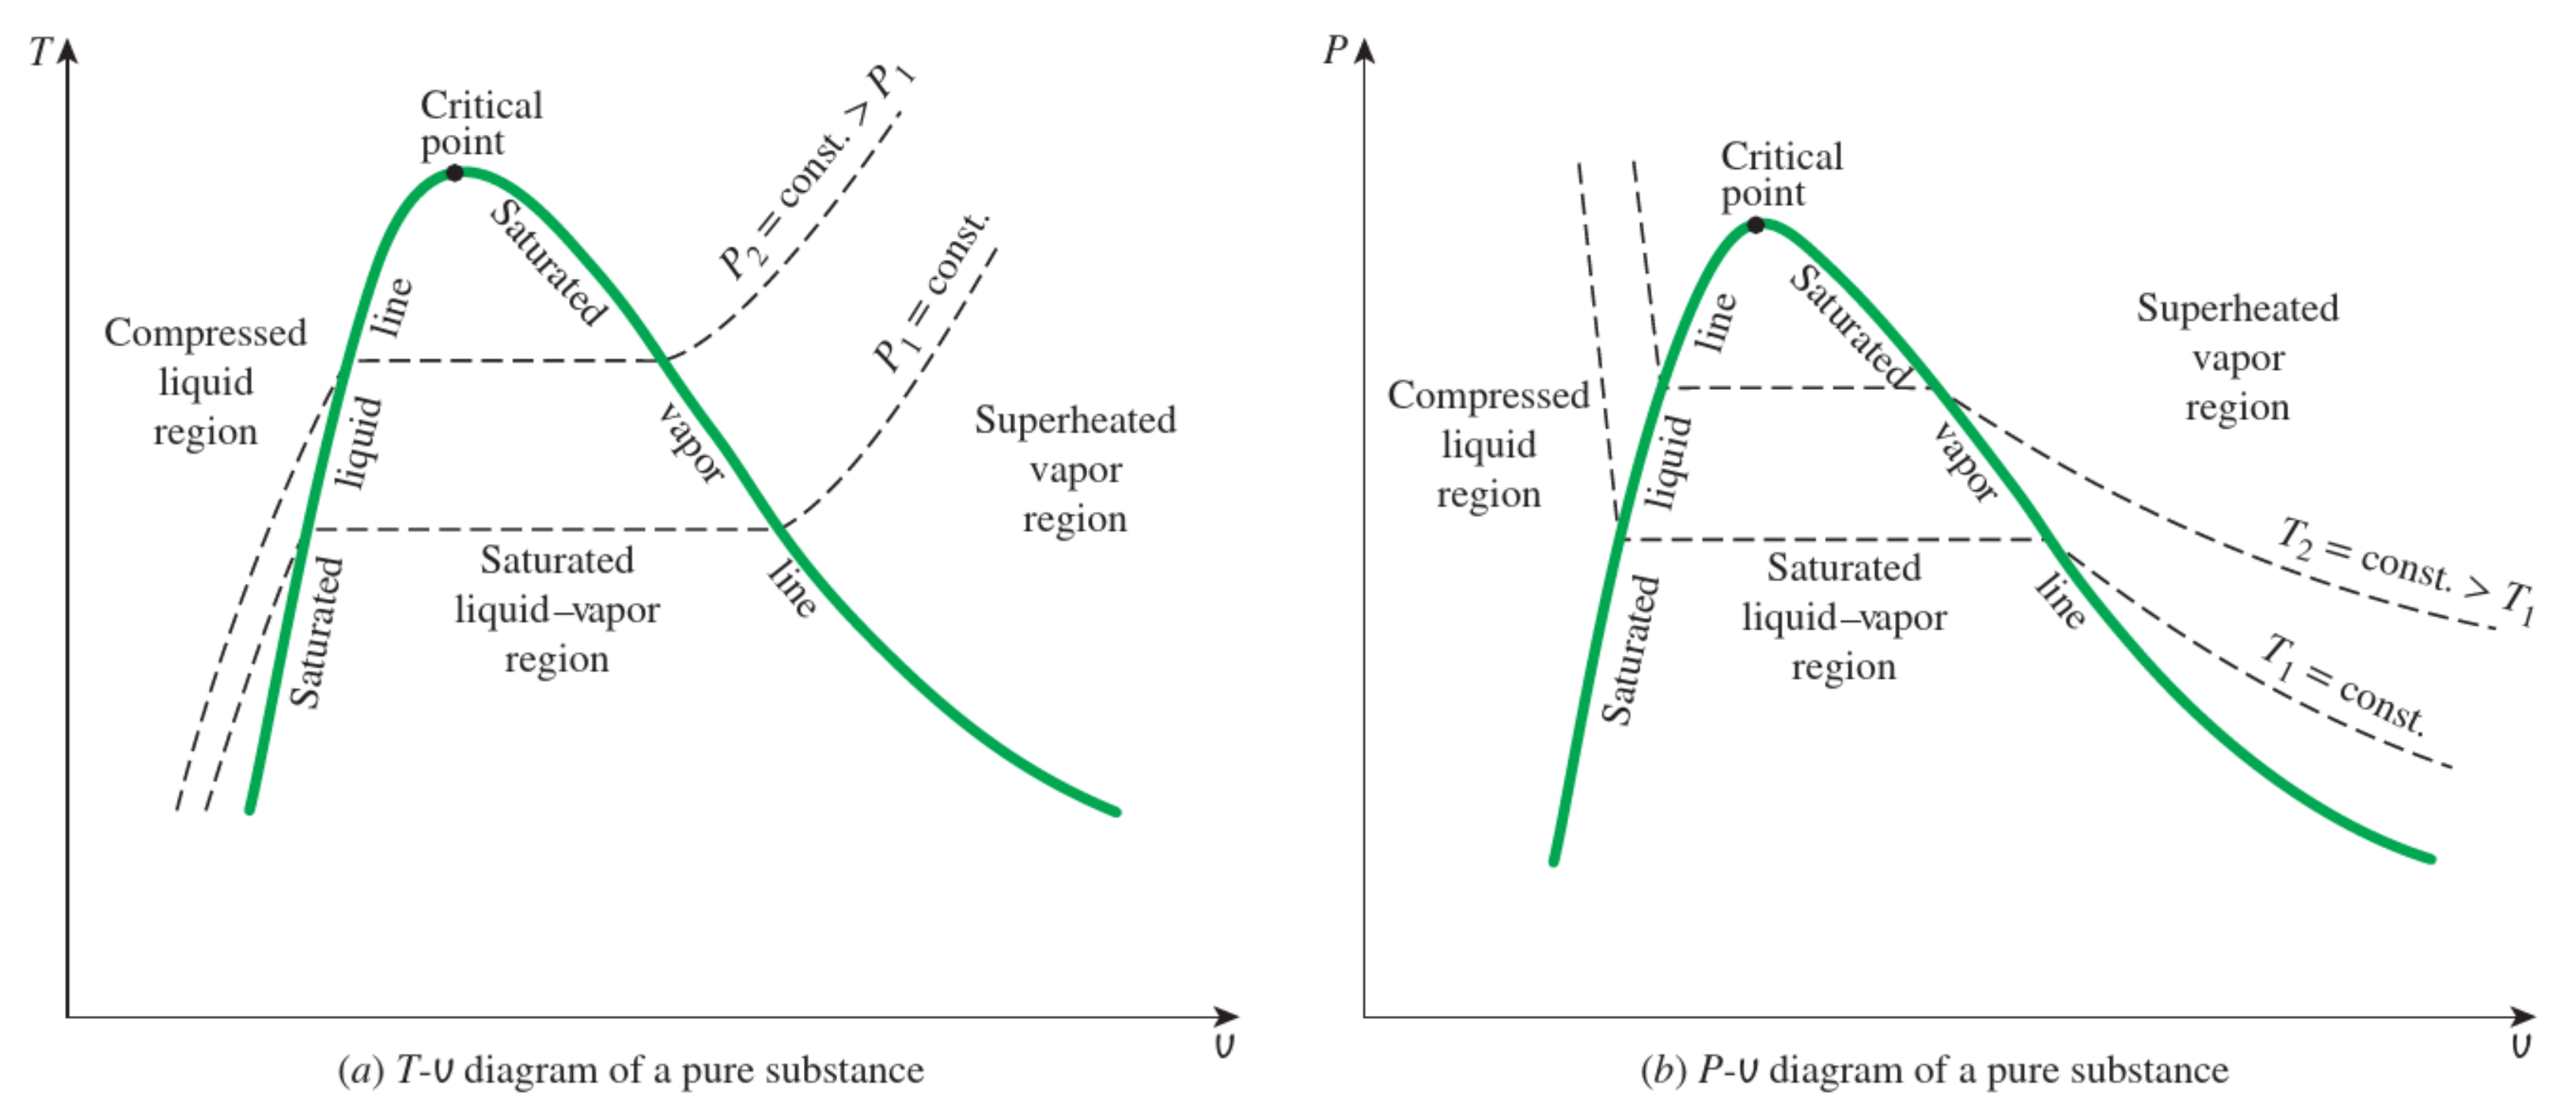
\includegraphics[width=\textwidth]{Images/thermo1.png}
\end{center}

The isolines show constant pressures or temperatures respectively. Importantly, holding pressure or temperature constant under the dome necessarily holds the other quantity constant.

%\newpage

\begin{shaded}
In general, an intensive property $p$ (standing in for volume, enthalpy, internal energy, etc) of a system are related to pressure and temperature by:
\begin{itemize}
    \item[] \textbf{Compressed liquid}: $p\approx p_{f}$ at $T$. Properties of a liquid at fixed temperature vary negligibly.
    \item[] \textbf{Saturated liquid}: $p=p_f$ from a property table.
    \item[] \textbf{Liquid-vapor mixture}: $p=p_f + x(v_g-v_f)$, where $x$ is the \textbf{quality} of the mixture, defined by the mass ratio of vapor to total mass: \[x=\frac{m_{\text{vapor}}}{m_\text{liquid}+m_\text{vapor}}\] Quality directly corresponds to a position along the horizontal portion of an isoline under the dome.
    \item[] \textbf{Saturated vapor}: $p=p_g$ from a property table.
    \item[] \textbf{Superheated vapor}: read from a property table for most values.
\end{itemize}
\end{shaded}

In absence of property tables, the \textbf{ideal gas law} sometimes provides a decent approximation for the behavior of gases. In particular, the ideal gas law is given by the equivalent relationships \[Pv=RT\hspace{0.325in}\text{or}\hspace{0.325in}PV=mRT\hspace{0.325in}\text{or}\hspace{0.325in}PV=nR_uT\] where $R$ is the gas constant for a specific substance and $R_u$ is the universal gas constant. Under certain conditions, a gas deviates from ideal behaviors. In this case, a \textbf{compressibility factor} $Z=v_\text{real}/v_\text{ideal}$ adjusts the ideal gas law: \[Pv=ZRT\] $Z$ is generally read from a compressibility chart (where $P_\text{cr}$ and $T_\text{cr}$ are particular to a substance and read from a table):
\begin{center}
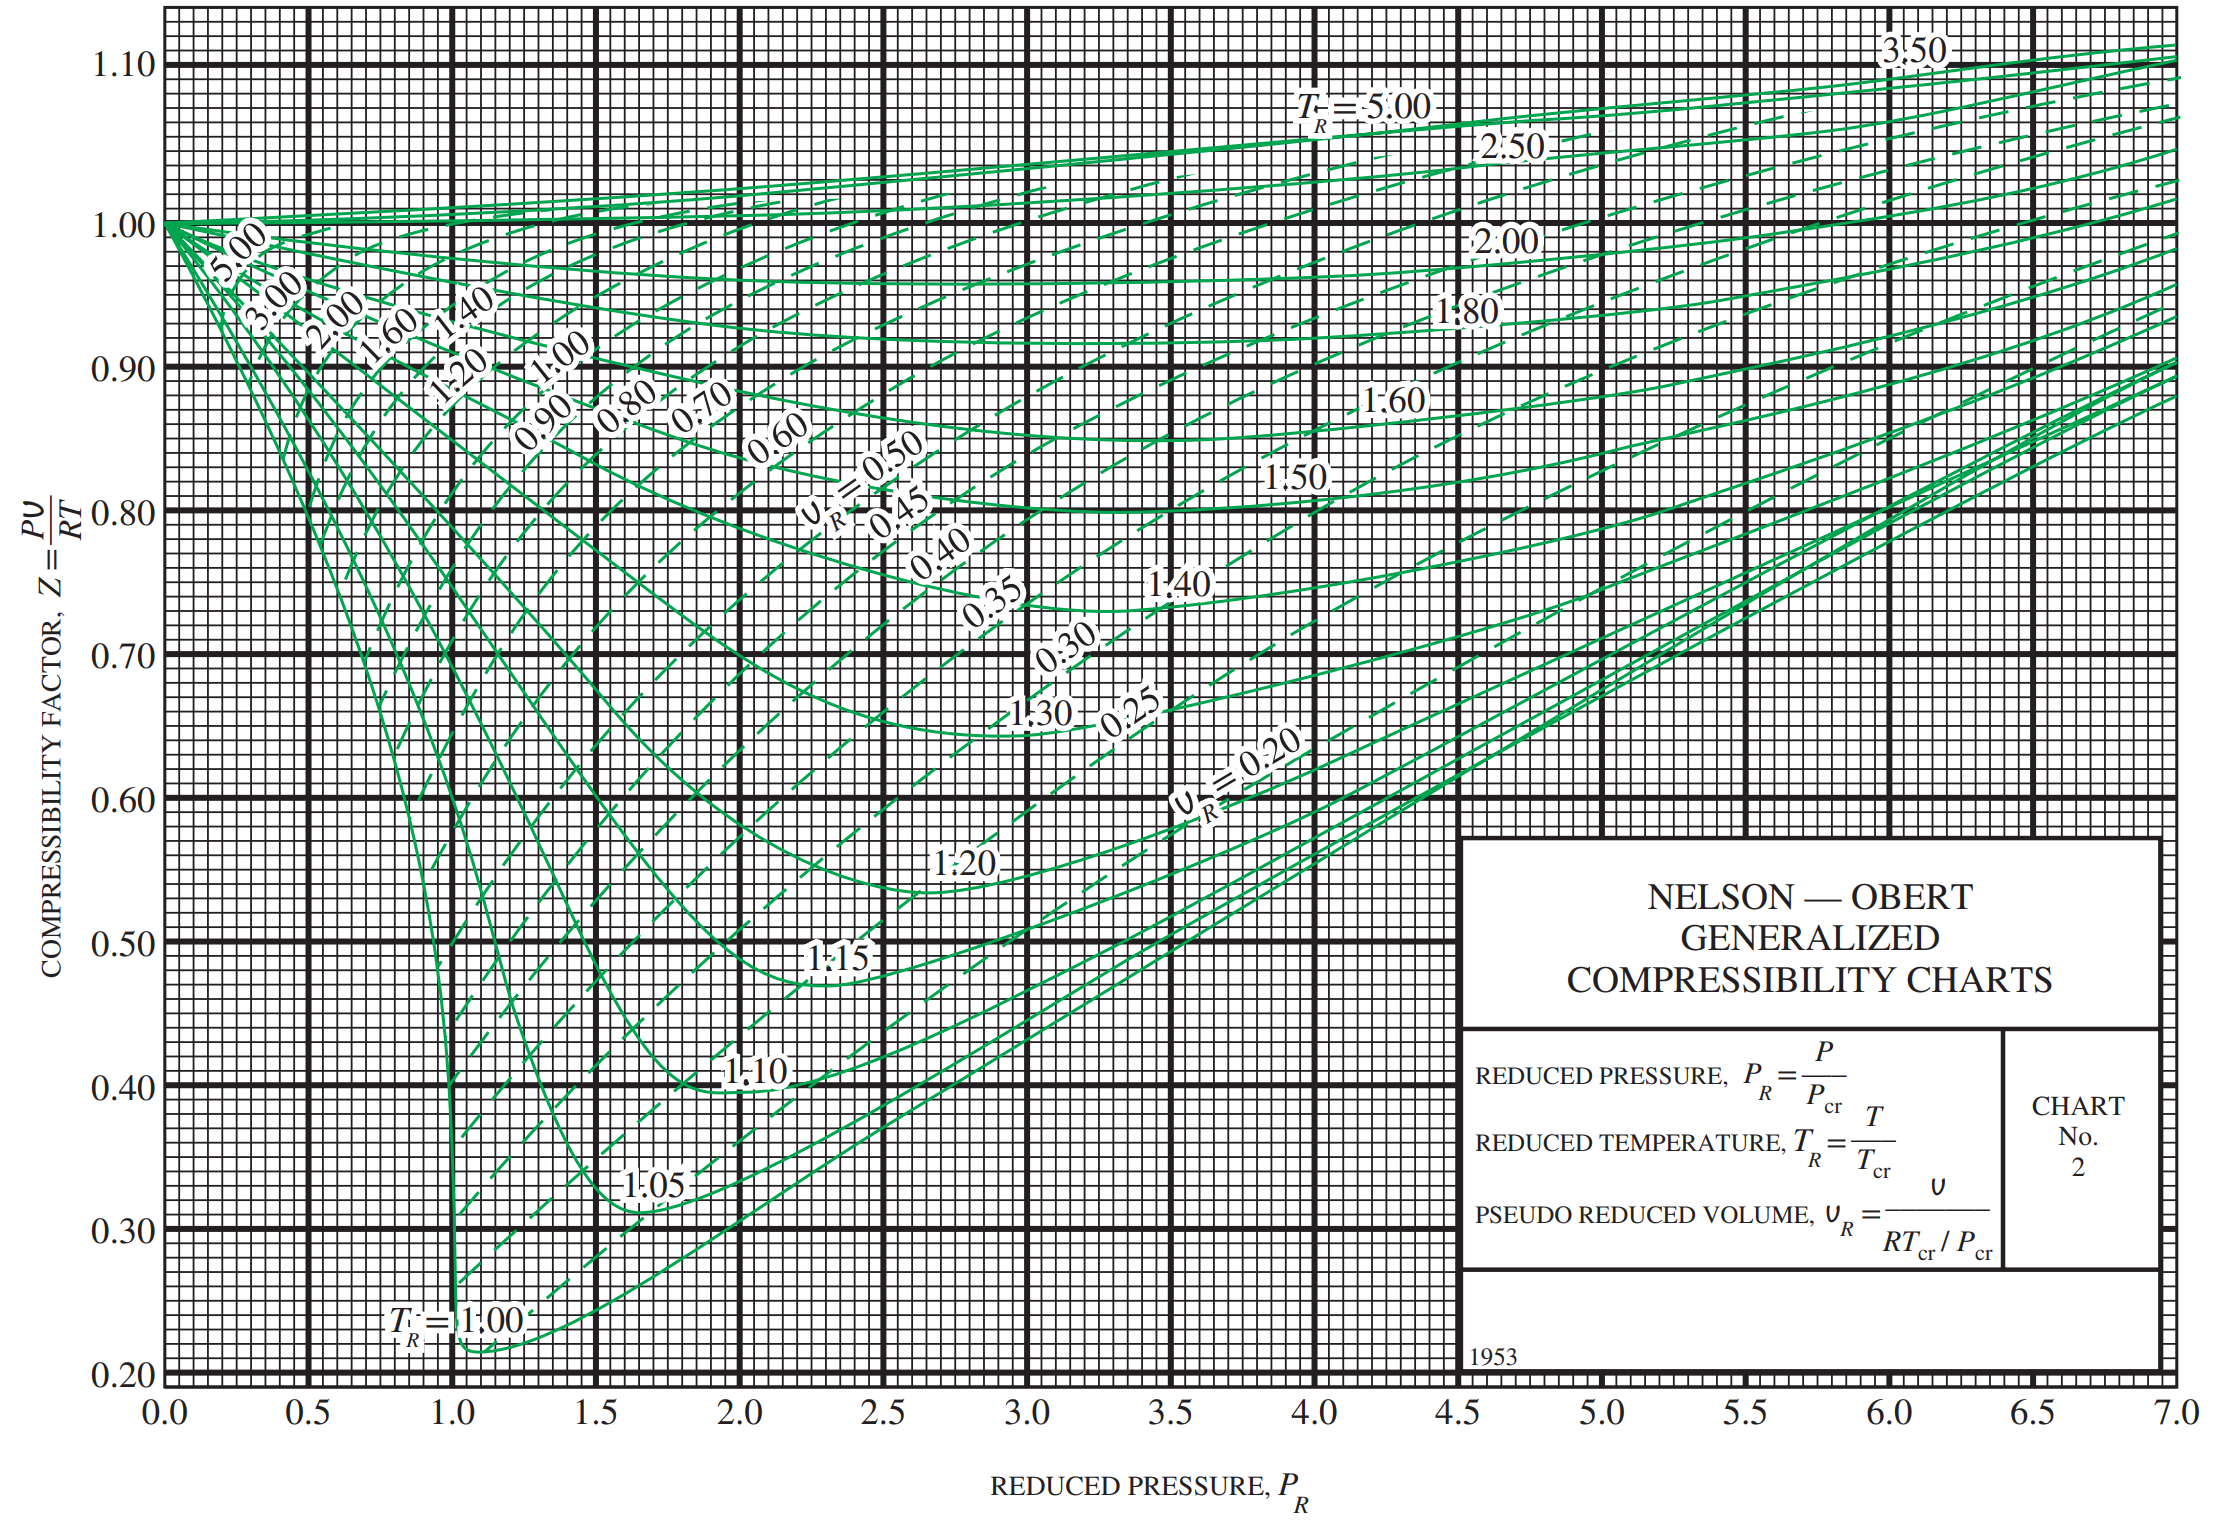
\includegraphics[width=0.85\linewidth]{Images/thermo2.png}
\end{center}

\begin{shaded}
    A gas is generally "ideal" (the ideal gas law is a reasonable approximation) under any of the following conditions:
    \begin{enumerate}
        \item Pressure is low: $P_{R}<<1$ (irrespective of temperature).
        \item Temperature is high: $T_R > 2$ (irrespective of pressure).
        \item $Z > 0.9$
    \end{enumerate}
\end{shaded}

\subsection{Energy Analysis of Closed Systems}

In a closed system, mass does not transfer across the system boundary. For these systems, energy analysis simply involves energy balance and an analysis of the temperature, pressure, and volume changes in the system.

\textbf{Boundary work} (also known as \textit{moving boundary work}) involves the \textit{compression} or \textit{expansion} of a system boundary, such as in a piston. In the case of a piston, pressure remains constant because the weight of the piston head pushes on the gas in the piston with constant force and area, so only volume changes between states. From the definition of mechanical work, the boundary work done moving a piston (or any other boundary) is given by \[\Delta W_B = F\Delta x = PA\Delta x = P\Delta V\] Most generally, total boundary work $W_B$ may be found by integration: \[W_B = \int_{V_1}^{V_2} PdV\]
Using this definition, it is possible to derive an expression for the boundary work of various common processes:

\begin{shaded}
    \begin{enumerate}
        \item \textbf{Boundary Work for Constant Volume (Isochoric) Process}. $\Delta V = 0$, so \[W_{B\text{, const. }V} = 0\]
        \item \textbf{Boundary Work for Constant Volume (Isobaric) Process.} $P$ is a constant and not a function of $V$, so it may be pulled out of the integral: \[W_{B\text{, const. }P} = P\int_{V_1}^{V_2} dV = P(V_2-V_1)\]
        \item \textbf{Boundary Work for Constant Temperature (Isothermal) Process.} Assuming ideal gas, $PV$ is a constant. So, let $PV=C\implies W_B = \int_{V_1}^{V_2}\frac{C}{V}dV = C\ln\left(\frac{V_2}{V_1}\right)$. But $C=P_1V_1$ or $C=P_2V_2$ or $C=mRT$ because all three are equivalent given ideal gas with constant temperature, so \[W_{B\text{, const. }T} = P_1V_1 \ln\left(\frac{V_2}{V_1}\right) = P_2V_2 \ln\left(\frac{V_2}{V_1}\right) = mRT \ln\left(\frac{V_2}{V_1}\right)\]
        \item \textbf{Boundary Work for Polytropic Process.} A polytropic process has $PV^k = C$ for some constant $k$ and $C$. Given $k=1$ (ideal gas), this is simply the isothermal case. For $k\neq 1$, integration gives \[W_{B\text{, polytropic}} = \frac{P_2V_2 - P_1V_1}{1-k} = \frac{mR(T_2 - T_1)}{1-k}\]
    \end{enumerate}
\end{shaded}

For a process, work is given visually by the area under the curve on a $P$-$v$ diagram. For a process which is a cycle, net work $W_{net}$ is given by the area enclosed by the process curves. Boundary work should be \textit{negative for compression} (work is an input) and \textit{positive for expansion} (work is an output).

\textbf{Specific heat} is a measure of the energy required to raise the temperature of a unit mass of a substance by one degree. In general, thermodynamics considers specific heat at \textit{constant volume} $c_v$ and specific heat at \textit{constant pressure} $c_p$. Formally, specific heats are given by the following differentials:
\[c_v = \left(\pd{u}{T}\right)_{v=\text{const}}\hspace{1in}c_p = \left(\pd{h}{T}\right)_{P=\text{const}}\]
For ideal gases, both $u$ and $h$ are functions of temperature alone, so these differentials become exact: \[\frac{du}{dT} = c_v(t)\hspace{1in} \frac{dh}{dT} = c_p(T)\] Thus, \[\Delta u = u_2 - u_1 = \int_{T_1}^{T_2}c_v(T)dT\hspace{1in}\Delta h = h_2 - h_1 = \int_{T_1}^{T_2}c_p(T)dT\]
where $c_v$ and $c_p$ are generally polynomials with exact equations available in a property table. For some temperature ranges, $\Delta u$ and $\Delta h$ may be approximated by
\[ \Delta u \approx c_{v,avg}\Delta T,\hspace{0.5in}\Delta h \approx c_{p,avg}\Delta T\]

For incompressible substances (liquids and solids), pressures and specific volumes are constant, so $c_p = c_v = c$. Thus, change in internal energy for a liquid or solid is given by \[\Delta u \approx c_{avg}\Delta T\]

\subsection{Energy Analysis of Open Systems (Control Volumes)}

In an open system, a fixed control volume is considered where both mass and energy may be transferred across the system boundary. Like energy, mass is a conserved quantity with a conservation law. 
\begin{shaded}
    \textbf{Conservation of mass}. Given a constant volume, \[m_\text{in,net} - m_\text{out,net} = \Delta m\hspace{0.5in}\text{kg}\] In (differential) rate form, \[\dot m_\text{in,net} - \dot m_\text{out,net} = \frac{dm}{dt}\hspace{0.5in}\text{kg}/\text{s}\]
\end{shaded}

If mass changes with time, there is some \textbf{mass flow rate}, given by \[\dot m = \rho \vec{v}_{avg} A = \rho\dot V = \frac{\dot V}{v}\] Here, $\vec{v}_{avg}$ is the magnitude of the average velocity, $v$ is specific volume, and $A$ is the cross-sectional area through which the mass is flowing. The \textbf{volume flow rate} is then given by \[\dot V = \vec{v}_{avg} A\]

Many open systems, such as power plants, operate in \textbf{steady flow} (i.e. mass flow rate does not vary considerably with time). In this case, it is assumed that $\Delta \dot m=0$, yielding $\dot m_{\text{in,net}} = \dot m_\text{out,net}$

For an open system, the general energy balance is given by \[\dot Q_\text{in} + W_\text{in} + \sum_\text{in} \dot m(h +\vec{v}^2/2 + gz) = \dot Q_\text{out} + \dot W_\text{out} + \sum_\text{out}\dot m(h + \vec{v}^2/2 + gz)\]

For a particular system, many of these quantities are negligible. In particular, kinetic and potential energies are neglected in many systems, and insulated systems may take $\dot Q_\text{in} = \dot Q_\text{out} = 0$. Similar analysis can be used to reach an energy balance for any system.

\subsection{Entropy}

The Second Law of Thermodynamics describes the direction of spontaneous change for a system. In particular, the Second Law relates to processes operating between two different \textbf{thermal reservoirs} (external bodies, large enough that their temperature is roughly constant; i.e. the atmosphere, rivers, etc). Some cyclic devices of interest (and their ideal, reversible (Carnot) counterparts) are outlined:

\begin{itemize}
    \item[] \textbf{Heat engine} (i.e. a steam engine): cyclic process where heat is taken from a high temperature source, converted partially into work, and the rest rejected into a low-temperature sink. Thermal efficiency given by \[\eta_\text{thermal} = \frac{W_\text{net,out}}{Q_\text{out}} = \frac{Q_\text{in}-Q_\text{out}}{Q_\text{in}}\ \longrightarrow \eta_\text{Carnot} = \frac{T_H-T_L}{T_H}\] Construction of a heat engine is mechanically limited by the Kelvin-Planck Statement: \begin{shaded}
\textbf{Kelvin-Planck Statement}:

It is impossible for any device that operates on a cycle to receive heat from a single reservoir and produce a net amount of work.
\end{shaded}

\item[] \textbf{Refrigerators}: cyclic process where work is added to a system to remove heat. Thermal efficiency is given by a coefficient of performance: \[\text{COP}_R = \frac{Q_\text{Low}}{W_\text{net,in}} = \frac{Q_\text{Low}}{Q_\text{High}-Q_\text{Low}}\longrightarrow \eta_\text{Carnot} = \frac{T_L}{T_H-T_L}\] Construction of a refrigerator is limited by the Clausius Statement: \begin{shaded}
    \textbf{Clausius Statement}:
Is it impossible to construct a device that operates in a cycle and produces no effect other than the transfer of heat from a lower-temperature body to a higher-temperature body.
\end{shaded}

\item[] \textbf{Heat Pumps}: cyclic process where work is added to a system to generate heat. Thermal efficiency is given by a coefficient of performance: \[\text{COP}_{HP} = \frac{Q_\text{High}}{W_\text{net,in}} = \frac{Q_\text{High}}{Q_\text{High}-Q_\text{Low}}\longrightarrow\eta_\text{Carnot} = \frac{T_H}{T_H-T_L}\]
\end{itemize}

A process is \textbf{irreversible} if the process cannot be spontaneously undone. Irreversibility may be introduced in real processes by friction, electrical resistance, mixing of fluids, etc.

\begin{shaded}
 \textbf{Carnot Principle}.
The efficiency of an irreversible process is always less than the efficiency of a reversible one (Carnot) operating between the same two reservoirs. Carnot efficiency is upper bound.
\end{shaded}

Entropy is introduced as a measure of irreversibility. Change in entropy for a (cyclic) process is given by \[\Delta S = S_2 - S_1 = \oint \frac{dQ}{T}\] where \[\oint \frac{d Q}{T}\leq 0\text{ always (\textbf{Clausius Inequality})}\] 

\newpage

The Second Law of Thermodynamics emerges from this definition of entropy: \begin{shaded}
     \textbf{Second Law of Thermodynamics}.
     Entropy cannot decrease during a process; entropy generated internally in a process is either zero or positive.
     \[S_{gen} \geq 0\] where \[S_\text{gen}\begin{cases}
        > 0 \implies \text{irreversible process}\\
        = 0 \implies \text{reversible process}\\
        < 0 \implies \text{impossible process}
     \end{cases}\]
 \end{shaded}

 For a process, entropy balance is given by \[S_\text{in} - S_\text{out} + S_\text{gen} = \Delta S_\text{system}\]

Entropy change is related to heat generation. Rearranging the differential form of the Clausius Inequality gives: \begin{eqnarray*}
    \frac{dQ}{T} = dS &\implies& dQ = TdS\\
    &\implies& Q = \int_{T_1}^{T_2} TdS\hspace{0.125in}\text{ (area under $T$-$s$ graph)}
\end{eqnarray*}

For mechanical processes, entropy is generally changed through the addition of heat. At a microscopic level (in statistical thermodynamics), entropy increases as the "disorder" of a system increases. The following may increase disorder in a system:
 \begin{enumerate}
     \item[] \textbf{Change of volume}: molecules have more space to move, causing more disorder (i.e. expansion of a gas). 
     \item[] \textbf{Change of composition}: Some compositions are more "chaotic" than others (i.e. a crystalline structure is less chaotic than a gaseous state)
     \item[] \textbf{Change of temperature}: temperature is a measure of average molecule velocity. Higher temperatures mean higher velocities and therefore greater disorder.
 \end{enumerate}

The Boltzmann Postulate gives an exact value for entropy relying on statistical mechanics: \begin{shaded}
\textbf{Boltzmann Postulate} (statistical thermodynamics).
 \[S = k\ln W\] where $W$ is the number of microstates and $k$ is the Boltzmann constant.
\end{shaded}

Because entropy is defined in terms of microstates, entropy is an \textbf{intensive property} of a system. The limiting case of the Boltzmann Postulate, with $W=1$, sets the reference point for zero entropy and comprises the Third Law of Thermodynamics:

\begin{shaded}
    \textbf{Third Law of Thermodynamics} A pure crystalline substance at absolute zero temperature is in perfect order, and its entropy is zero.
\end{shaded}

For an ideal gas, change in entropy is given by \[\Delta S_\text{ideal gas} = \underbrace{c_v \ln (T_2 / T_1) + R\ln (V_2 / V_1)}_{c_v\text{ at average temperature}} =\underbrace{c_p\ln (T_2 / T_1) - R\ln (P_2 / P_1)}_{c_p\text{ at average temperature}}\]

And for a solid or liquid, change in entropy is given by \[\Delta S = c_{avg}\ln(T_2/T_1)\]

For an ideal gas, isentropic processes are polytropic with $k=c_p/c_v$. The equations for an isentropic process are given:

\[\left(\frac{T_2}{T_1}\right)_{s=\text{const}} = \left(\frac{v_1}{v_2}\right)^{k-1}\]

\[\left(\frac{T_2}{T_1}\right)_{s=\text{const}} = \left(\frac{P_2}{P_1}\right)^{(k-1)/k}\]

\[\left(\frac{P_2}{P_1}\right)_{s=\text{const}} = \left(\frac{v_1}{v_2}\right)^{k}\]

\textbf{Isentropic efficiency} is a measure of how far a real process deviates from its ideal efficiency. Isentropic efficiencies for various common devices are given outlined:

\[\eta_{\text{turbine}} = \frac{W,\text{ actual turbine}}{W,\text{ isentropic turbine}} = \frac{W_a}{W_s} \approx \frac{h_1-h_{2a}}{h_1-h_{2s}}\]

\[\eta_{compressor} = \frac{\text{isentropic compressor work }W_s}{\text{actual compressor work }W_a} = \frac{h_{2s}-h_1}{h_{2a}-h_1} = \underbrace{\frac{V(P_2-P_1)}{h_{2a}-h_1}}_\text{Pumps only (liquids)} 
\]

\subsection{Power Cycles} % mod 8 is gas power cycle, mod 9 is vapor power cycles

Many important power-producing devices operate on a cycle. Two distinct types of cycles, relevant to everyday energy production, are of interest: gas power cycles, as is typical in engines, and vapor power cycles, as is typical in power plants.

For every cycle, the energy balance reduces to $Q_\text{net}-W_\text{net} = 0$, or $Q_\text{net} = W_\text{net}$. Thus, it is possible to analyze the net output of a cycle either using heat (on a $T$-$s$ diagram) or work (on a $P$-$v$ diagram). In each cycle analyzed, thermal efficiency is given as a ratio of \textit{net work} to \textit{heat in}: \[\eta = \frac{W_\text{net}}{Q_\text{in}}\]

The \textbf{gas power cycles} listed here operate on the \textbf{air-standard assumptions}, which allow the processes to be simplified for analysis:

\begin{shaded}
\textbf{Air-Standard Assumptions}.
\begin{enumerate}
    \item The working fluid is air, which circulates through the system in a closed loop as an ideal gas.
    \item All processes in the cycle are internally reversible.
    \item Combustion processes are replaced by heat-addition from an external source.
    \item Exhaust processes are replaced by heat-rejection which returns the air to its initial state.
\end{enumerate}
\end{shaded}

\newpage

Air-standard assumptions are used in analysis of engines. Several cycles are listed below:

\begin{enumerate}
    \item[] \textbf{Otto Cycle}. Gasoline engines operate on the Otto cycle using an air-fuel mixture, generally approximated as air for the purposes of analysis. The Otto cycle has four distinct steps:
    \begin{enumerate}
        \item Compression Stroke (replaced by isentropic compression)
        \item Power (expansion) Stroke (replaced by constant volume heat addition)
        \item Exhaust Stroke (replaced by isentropic expansion)
        \item Intake Stroke (replaced by constant volume heat rejection)
    \end{enumerate}
    \begin{center}
        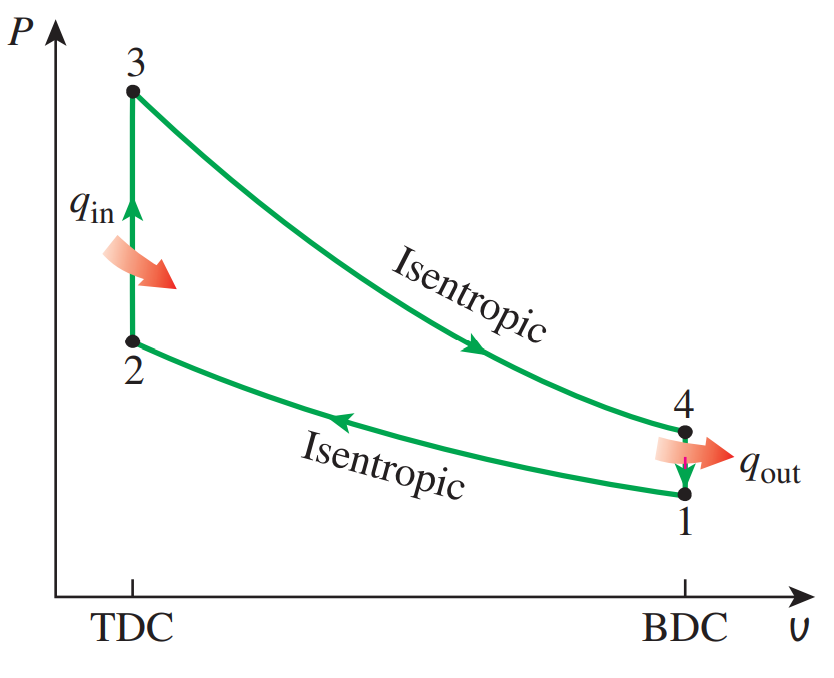
\includegraphics[width=0.4\linewidth]{Images/thermo otto.png}
    \end{center}
    Efficiency for an Otto cycle is given by \[\eta = 1 - \frac{1}{r^{k-1}},\hspace{0.5in}r:=\frac{V_\text{max}}{V_\text{min}},\hspace{0.1in} k:=c_p/c_v\]
    The Otto cycle is limited by \textit{autoignition}, or \textit{engine knock}. For large compression ratios $r$ (around $12$), pockets of fuel-air mixture have a tendency to ignite before the power stroke, causing an effective reduction in volume ratio and reducing efficiency.

    \item[] \textbf{Diesel Cycle}. Diesel engines operate on the Diesel cycle, where air is compressed to high temperatures before pure Diesel fuel is injected and combusted due to the high pressure and high temperature. The Diesel cycle also have four distinct steps:
    \begin{enumerate}
        \item Compression Stroke (replaced by isentropic compression)
        \item Combustion (fuel injection) Stroke (replaced by constant pressure heat addition)
        \item Exhaust Stroke (replaced by isentropic expansion)
        \item Intake Stroke (replaced by constant volume heat rejection)
    \end{enumerate}
    \begin{center}
        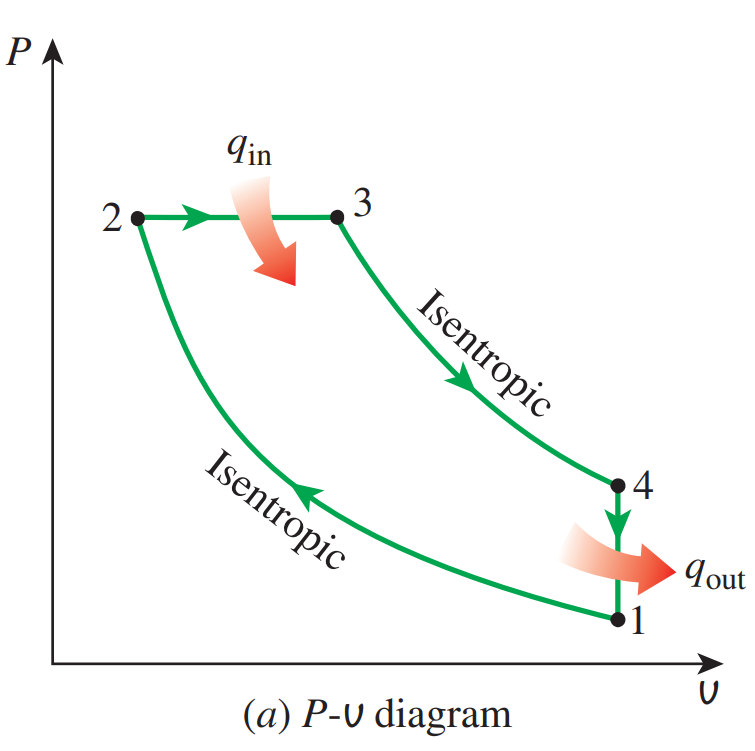
\includegraphics[width=0.4\linewidth]{Images/thermo diesel.png}
    \end{center}
    Efficiency for a Diesel cycle is given by \[\eta = 1-\frac{1}{r^{k-1}}\left[\frac{r_c^k - 1}{k(r_c-1)}\right],\hspace{0.5in}r_c:=\frac{V_3}{V_2}\]
    The Diesel cycle always has a lower efficiency as the same compression ratio, but because combustion is initiated by fuel injection, autoignition is not a concern in Diesel engines and Diesel engines can reach higher raw efficiencies than an engine operating on the Otto cycle.
    \item[] \textbf{Brayton Cycle}. Gas-turbine engines, such as those used in propulsion aircraft, generally operate on a Brayton cycle. A Brayton Cycle uses four devices, and the cycle has four distinct steps:
    \begin{enumerate}
        \item Compressor (isentropic compression)
        \item Heat Exchanger (constant-pressure heat addition)
        \item Turbine (isentropic expansion)
        \item Heat Exchanger (constant-pressure heat rejection)
    \end{enumerate}
    \begin{center}
        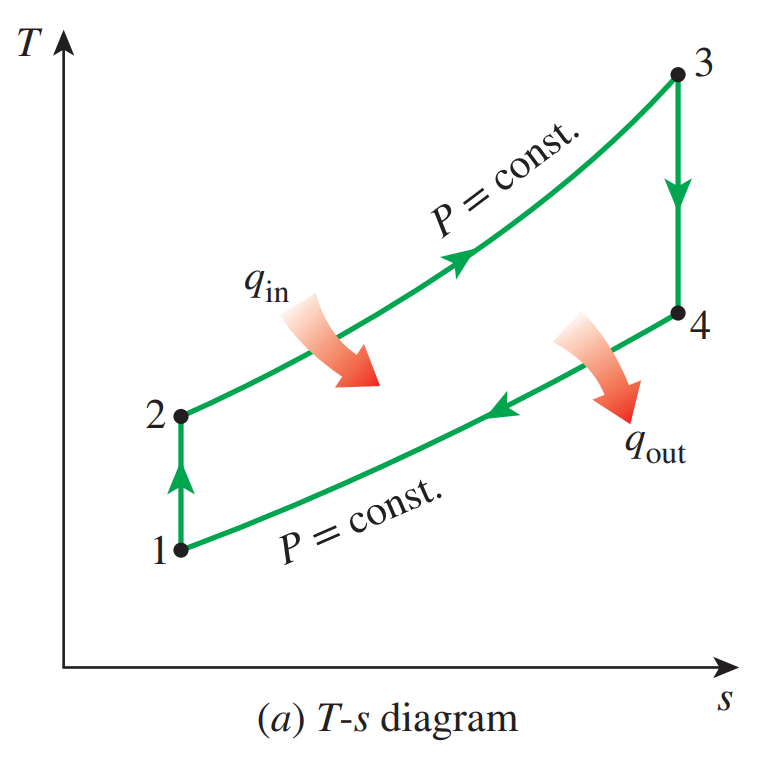
\includegraphics[width=0.4\linewidth]{Images/thermo brayton.png}
    \end{center}
    Efficiency for a Brayton Cycle is given by \[\eta = 1-\frac{1}{r_p^{(k-1)/k}},\hspace{0.5in}r_p=\frac{P_2}{P_1}\] Typical pressure ratios $r_p$ for a Brayton cycle are between $5$ and $20$.
\end{enumerate}

\newpage

Many power plants operate on some form of vapor power cycle, utilizing the phase change of water into steam to produce useful work. The Rankine Cycle is a simple, common cycle utilizing water.

\begin{enumerate}
    \item[] \textbf{Rankine Cycle}. An ideal Rankine cycle utilizes four devices and water in both liquid and vapor form to produce power:
    \begin{enumerate}
        \item Pump (isentropic compression of liquid, initially saturated liquid)
        \item Boiler (constant pressure heat addition to superheated vapor)
        \item Turbine (isentropic expansion)
        \item Condenser (constant-pressure heat rejection)
    \end{enumerate}
    \begin{center}
        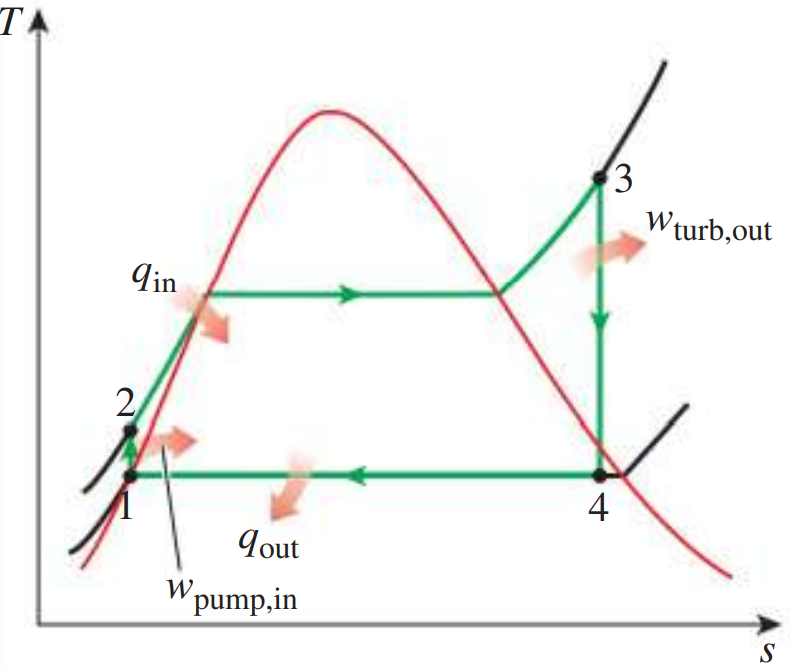
\includegraphics[width=0.4\linewidth]{Images/thermo rankine.png}
    \end{center}
    The efficiency of a Rankine Cycle is given by \[\eta = 1 - \frac{Q_\text{out}}{Q_\text{in}}\] The efficiency of a Rankine cycle may be improved by adding regeneration, diverting some warm water to effectively reduce $Q_\text{in}$.
\end{enumerate}

For power cycles, the \textbf{backwork ratio} is another measure related to efficiency. Backwork ratio is given by \[\text{BWR} = \frac{W_\text{in}}{W_\text{out}}\] Backwork ratio measures what fraction of the output work must be used to power the cycle (in raising the piston, powering the compressor, etc).
\section{Statics and Mechanics of Materials}

\begin{center}
    Notes from \textbf{MECHENG 211: Introduction to Solid Mechanics}

    Taken at University of Michigan, Winter 2025
\end{center}

\subsection{Static Equilibrium} %% Chapter 1-5/6

A force $\vec{F}$ creates a \textbf{moment} about a point if it is located a distance $\vec{r}$ from the line of action of the $\vec{F}$. The moment $\vec{M}$ of a force is perpendicular to both $\vec{F}$ and $\vec{r}$, so in two dimensions, $\vec{M}$ necessarily points into or out of the page and is given by \[M = Fr\] In three dimensions, moments are computed by a cross product. For a moment about a point $A$ produced by a force acting at point $B$, the moment $\vec{M}_A$ is given by \[\vec{M}_A = \vec{r}_{AB}\times \vec{F} = (\vec{r}_B-\vec{r}_A)\times \vec{F}\]

A body is in \textbf{static equilibrium} if it does not translate or rotate. For this to be the case, the vector sum of the forces acting on the body must be zero, and the vector sum of the moments about any point on the body must also be zero. 

At each \textit{support} contacting a body, the body produces a \textit{reaction force}. For a body to be fully constrained, there must be as many reaction forces as \textit{degrees of freedom}. In two dimensions, there are \textit{three degrees of freedom} ($x$ and $y$ translation, and a moment). In three dimensions, there are \textit{six degrees of freedom} (translation in $x$ $y$, $z$, and moments in $x$, $y$, and $z$).

Most supports fall into one of the following categories:
\begin{enumerate}
    \item[] \textbf{Fixed support}. Sometimes called a built-in support. Constrains motion and rotation in all directions and therefore produces reaction forces and reaction moments in all directions.
    \item[] \textbf{Pin support}. Constrains translational motion while allowing free rotation, therefore producing reaction forces in the horizontal and vertical directions. Pin supports may often be used to approximate joints in structures like beams and trusses.
    \item[] \textbf{Simple support}. Prevents motion normal to the point of contact, producing a single reaction force. This joint is mathematically equivalent to a roller.
\end{enumerate}

When bodies come into contact through \textit{compressive forces}, a frictional force $F$ opposes motion. The magnitude of frictional force is generally given by the inequality $|F| < \mu N$. \textit{Incipient slip} refers to the force required to begin motion of a body, occurring when the frictional forces have just barely been overcome.

\subsection{Composite Structures}

It is possible to analyze a complicated, multi-element structure by breaking it into its components and supports. Such analysis involves drawing a free body diagram for each part, with external forces and reaction forces (and their 3rd Law reaction) listed at their appropriate positions and supports. Because the entire structure is in static equilibrium, each component must also be in static equilibrium and the forces on each component must thus satisfy the static equilibrium conditions.

A \textit{two-force member} is any component loaded at only two points, such as a support member in a truss. In this case, \[\vec{F}_A + \vec{F}_B = \vec{0},\hspace{0.5in} \vec{r}_{AB}\times \vec{F}_B = \vec{0}\] so $\vec{F}_A = -\vec{F}_B$ and thus forces act \textit{along a single line} through the component. If the forces point outwards, the member is in \textbf{tension}; if the forces point inwards, the member is in \textbf{compression}.
\newpage
There are two main ways to analyze the internal forces in a determinate structure, such as a truss:
\begin{enumerate}
    \item[] \textbf{Method of Pins}. Most useful for solving systems where many or all internal forces are to be calculated. Steps: \begin{enumerate}
        \item[1.] Separate structure into separate two-force members.
        \item[2.] Draw free-body diagrams for each two-force member, approximating joints as pins with reaction forces pointing away (in tension, which is positive by convention).
        \item[3.] Solve the force balance for the desired internal forces. This involves (at most) an $x$ and $y$ force balance for each member.
    \end{enumerate}
    \item[] \textbf{Method of Sections}. Most useful for solving systems where only some internal forces need to be known. Steps:
    \begin{enumerate}
        \item[1.] Cut a section through the body, cutting through at most three elements with unknown internal forces. The internal forces from cut members become external forces for the remaining section.
        \item[2.] Draw a free-body diagram for the section in question, with unknown forces pointing away from cut members (in tension, which is positive by convention).
        \item[3.] Solve the force and moment balance for the section. Since the entire body is in equilibrium, the section must also be in equilibrium. This involves setting net forces in $x$ and $y$ and net moment equal to zero.
    \end{enumerate}
\end{enumerate}

Each section of a loaded body must experience internal reactions which balance the external forces and moments. If one were to make a cut through any section of the body, these reactions would be exactly what is required to support either section of the cut.

By convention, the internal reactions include a normal force $N$ acting perpendicular to the cut, a shear force $V$ acting parallel to the cut, and a moment $M$. The internal reactions have opposite orientations on opposite sides of the cut.

In three dimensions, there is a single normal vector $\vec{N}$, two directional components to $\vec{V}$ (i.e. $x$ and $y$), and three rotational components (a bending moment $\vec{M}$ about the $x$ and $y$ axis, and a twisting torque $T$ about the $z$ axis).

\subsection{Stress and Strain}

In general, \textbf{stress} refers to the force acting over an area on a body (i.e. a "pressure" over a surface), and \textbf{strain} refers to the deformation of the body. Normal stress is denoted $\sigma$ and shear stress is denoted $\tau$.

Given a normal force $N$ acting uniformly on an area $A$, the normal stress at the section is given by \[\sigma = \frac{N}{A}\] Moments may also impart a normal stress. In particular, for a bar with cross-sectional area $A$ and area moment of inertia $I_x$, there is an additional component of stress given by \[\sigma_{zz} = \frac{M_xy}{I_x} - \frac{M_yx}{I_y}\] where $x$ and $y$ are taken from the centroid $c=(\overline{x},\overline{y})$. Similarly, given a uniform shear force $V$, the (average) shear stress is given by \[\tau = \frac{V}{A}\] and torque on a bar can also produce additional shear stress: \[\tau = \frac{Tr}{J}\]

\newpage

Stress acting on a body produces a \textbf{strain}, or change in the dimensions of an object. When a bar is loaded with a tensile force, it may experience some extension from its initial length $L_0$, given by $\delta = L-L_0$. \textit{Normal strain} $\varepsilon$, or \textit{extensional strain}, is defined as the ratio of extension and initial length, given by \[\varepsilon = \frac{\delta}{L_0}\]

\textit{Shear strain} acting on a body is simply computed as the total change of angle $\phi_1$ with respect to the horizontal and $\phi_2$ with respect to the vertical: \[\gamma = \phi_1 + \phi_2\]

\textbf{Hooke's Law} may be generalized to any material, and directly relates stress and strain. \begin{shaded}
    \textbf{Multiaxial Hooke's Law}. For a material which is elastically (linearly) deformed, the strains on a material relate directly to the stresses acting on the material by Hooke's Law:

    \[\epsilon_x = \frac{\sigma_x}{E} - \frac{\nu\sigma_y}{E} - \frac{\nu \sigma_z}{E} + \alpha\Delta T\]
    \[\epsilon_y = \frac{\sigma_y}{E} - \frac{\nu\sigma_x}{E} - \frac{\nu \sigma_z}{E} + \alpha\Delta T\]
    \[\epsilon_z = \frac{\sigma_z}{E} - \frac{\nu\sigma_x}{E} - \frac{\nu \sigma_y}{E} + \alpha\Delta T\]

    Here, $E$ is Young's Modulus, and $\alpha$ is the coefficient of thermal expansion. Both are specific to a material. $\nu$ is \textbf{Poisson's Ratio}, the ratio by which compression in one direction results in extension in another, and is related to $E$ and $G$ by the relationship \[\nu = -\frac{\epsilon_\text{lateral}}{\epsilon_\text{axial}} = \frac{E}{2G} - 1\] More concisely, \[E = 2G(1+\nu)\] 
\end{shaded}

If a problem is \textit{statically indeterminate} (more unknowns than equations), another equation may be found by considering the extension or torsion in the body. In particular, for a beam built in at both ends, extension of the beam must be zero (both ends are fixed), giving a relation between forces. The same applies for a bar in torsion, with a relation between torques.

Extension is associated with normal strain. For a bar with area $A$, Young's Modulus $E$, and initial length $L_0$, the extension is given by: \[\delta = \frac{FL_0}{AE}\] 

A bar loaded with a torque $T$ has an analogous relationship to the extension of a bar. The angle of torsion, $\phi$, is given by \[\phi = \frac{TL}{JG}\] where $G$ is the shear modulus for a material and $J$ is the \textit{second moment of inertia}. For a cylindrical bar in torsion, the relation between torque, shear, and angle of torsion is as follows: \[\frac{T}{J} = \frac{\tau_{z}}{r}=G\frac{\phi_B-\phi_A}{L_{AB}}\]

\newpage

Thin-walled pressure vessels have an internal pressure $P$ (i.e. due to an internal gas or fluid) and a wall of thickness $t$, where $t$ is negligible compared to radius $r$.

\begin{enumerate}
    \item[] \textbf{Cylindrical pressure vessels}. Internal pressure $P$ with a cap on either end. Stresses are given by \[\underbrace{\sigma_\theta = \frac{Pr}{t}}_\text{hoop stress, tangent to walls},\hspace{0.5in}\underbrace{\sigma_\text{axial} = \frac{Pr}{2t}}_\text{longitudinal stress, normal to cap}\]
    \item[] \textbf{Spherical pressure vessels}. Internal pressure $P$ with symmetric hemispheres. Stresses are given by \[\underbrace{\sigma_\theta = \sigma_\phi = \frac{Pr}{2t}}_\text{tangent to walls}\]
\end{enumerate}

Superposition allows the addition of normal and shear stresses. Stresses emerge from loads applied to a body. For a coordinate system oriented (facing the surface) with $z$ normal to the surface, $y$ up, and $x$ left:

\begin{enumerate}
    \item[] \textbf{Normal stress}. May be imparted due to a moment or normal force. \[\sigma_{zz} = \frac{N}{A} + \frac{M_xy}{I_x} - \frac{M_yx}{I_y}\]
    \item[] \textbf{Shear stress}. May be imparted due to a torque or a shear force. \[\tau_{zy} = \frac{V_y}{A},\ \tau_{zx} = \frac{V_x}{A},\ \underbrace{\tau_{z\theta} = \frac{Tr}{J}}_\text{may be in $x$ or $y$}\]
\end{enumerate}

Note that other forces may be present, i.e. hoop stress or longitudinal stress if a pressure vessel is contributing support. It is necessary in such cases to identify the coordinate directions of any such stresses.

\subsection{Transformation of Stress and Strain}

For any element experiencing stresses, there exists a coordinate transformation to a \textit{principal axis} where all stress is normal stress and another transformation where all stress is shear stress. These axes are normal to each other. Fracture is most likely to occur along one of these axes, depending on the nature of the material.

In general, if an element experiences coordinate stresses $\sigma_x$, $\sigma_y$, and $\tau_{xy}$, then the stress in a new axis an orientation $\theta$ away is given by \[\sigma_{x'} = \frac{\sigma_x + \sigma_y}{2}+ \frac{\sigma_x - \sigma_y}{2}\cos 2\theta + \tau_{xy}\sin2\theta\]
    \[\sigma_{y'} = \frac{\sigma_x + \sigma_y}{2} - \frac{\sigma_x - \sigma_y}{2}\cos 2\theta - \tau_{xy}\sin2\theta\]
    \[\tau_{x'y'} = -\frac{\sigma_x -\sigma_y}{2}\sin2\theta + \tau_{xy}\cos2\theta\]

The stresses along the \textit{principal axis} may be found from these equations: \[\sigma_{1,2}=\frac{\sigma_x+\sigma_y}{2}\pm \sqrt{\left(\frac{\sigma_x-\sigma_y}{2}\right)^2 + \tau_{xy}^2}\] where $\sigma_1>\sigma_2$. The maximum shear stress in the plane is given by \[\tau_\text{max} = \sqrt{\left(\frac{\sigma_x-\sigma_y}{2}\right)^2 + \tau_{xy}^2}\] 
\newpage
\textbf{Mohr's circle} is a visual representation which may be constructed to visualize planar stress. \begin{shaded}
    \textbf{Construction of Mohr's Circle}. Mohr's circle may be constructed by the following steps: 
    \vspace{-1em}
    \begin{enumerate}
        \item Create coordinate axes, by convention positive stress to the right and positive shear to the bottom.
        \item Plot the center of the circle at $\frac{\sigma_x+\sigma_y}{2}$.
        \item Draw the circle with radius $\sqrt{\left(\frac{\sigma_x-\sigma_y}{2}\right)^2+\tau_{xy}^2}$.
        \item Optionally, plot the reference stresses $(\sigma_{x},\tau_{xy})$ as a reference point $\theta=0$. The angle $\theta_p$ to the principal axes may be determined by trigonometry.
    \end{enumerate}
\end{shaded}


Mohr's circle is drawn graphically as so: \begin{center}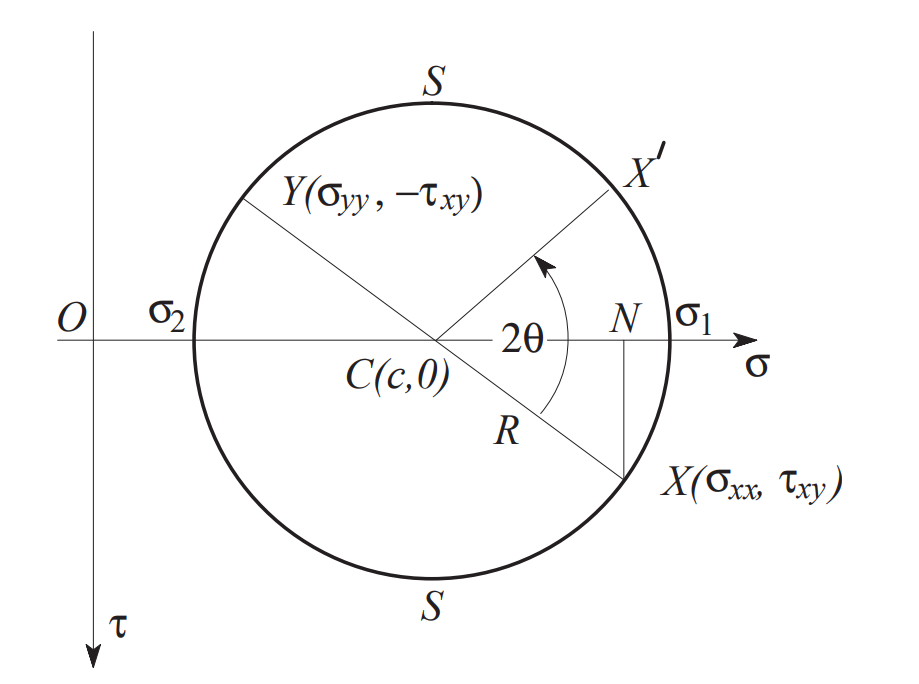
\includegraphics[scale=0.5]{Images/statics_mohrs.png}\end{center}

Since stress and strain are related by Hooke's Law, a Mohr's Circle may also be constructed for strain. The transformation equations are analogous to the stress transformations: \[\epsilon_{x'} = \frac{\epsilon_x + \epsilon_y}{2} + \frac{\epsilon_x-\epsilon_y}{2}\cos(2\theta) + \frac{\gamma_{xy}}{2}\sin(2\theta)\]
    \[\epsilon_{y'} = \frac{\epsilon_x + \epsilon_y}{2} - \frac{\epsilon_x-\epsilon_y}{2}\cos(2\theta) - \frac{\gamma_{xy}}{2}\sin(2\theta)\]
    \[\frac{\gamma_{x'y'}}{2} = - \frac{\epsilon_x-\epsilon_y}{2}\sin(2\theta) + \frac{\gamma_{xy}}{2}\cos(2\theta)\]

Principle strains also have an analogous transformations, and thus Mohr's circle is constructed in effectively the same manner for strains as with stresses:

\[\epsilon_{1,2} = \frac{\epsilon_x+\epsilon_y}{2}\pm \underbrace{\sqrt{\left(\frac{\epsilon_x-\epsilon_y}{2}\right)^2 + \left(\frac{\gamma_{xy}}{2}\right)^2}}_{\gamma_{\text{max}}/2}\]

It is important to note that, for planar stresses, $\sigma_3 = \sigma_z = 0$, but this is \textit{not the case} with planar strains, as a strain in one direction also causes strain in the others.

By using a \textit{strain gauge}, which measures electrical resistance (and thus strain, as electrical resistance increases with strain), the strain in a particular direction is related as follows:

\[\epsilon_a = \epsilon_x\cos^2\theta_a + \epsilon_y \sin^2\theta_a + \gamma_{xy}\sin\theta_a\cos\theta_a\]

Here, $\epsilon_a$ is read by the gauge and is thus known, and $\theta_a$ is known by the position of the strain gauge, so there are three unknowns. Thus, a strain gauge \textit{rosette}, with at least three strain gauges in unique directions, is required to find all the principal strains.

\subsection{Beam Deflection}

A loaded beam experiences some deflection, $u(z)$, as a function of the distance $z$ along the beam. For relatively small deflections, the following relationship holds: \[\frac{M(z)}{EI} = \frac{d\theta}{dz} = \frac{d^2u}{dz^2}\] $EI$ is the rigidity of the beam, and $M$ may vary as a function of position $z$. Integration gives $\theta(z)$ and $u(z)$ with constants of integration. These constants may be determined by evaluating $\theta$ or $u$ at supports and considering the boundary conditions of each support. Common boundary conditions, for support at arbitrary position $z=L_0$, are outlined:
\begin{enumerate}
    \item[] \textit{Built-in support}. \(u(L_0) = 0,\ \theta(L_0)=0\)
    \item[] \textit{Simple support}. \(u(L_0) = 0,\ M(L_0) = 0\)
    \item[] \textit{Free end}. \(V(L_0) = 0,\ M(L_0) = 0\)
\end{enumerate}
\section{Dynamics and Vibrations}

\begin{center}
    Notes from \textbf{MECHENG 240: Introduction to Dynamics and Vibrations}

    Taken at University of Michigan, Winter 2025

    using \textit{Dynamics}, by Meriam and Kraige
\end{center}

\subsection{Particle Kinematics} %%% 2.1 -- 2.7

Kinematics is the description of motion without reference to forces acting on an object. Particle kinematics is concerned with the movement of bodies which are physically small compared to their paths. 

For a particle a distance $s(t)$ from a fixed point in direction of unit vector $\hat e$, position may be defined by \[\vec{r}(t) = s(t)\hat e\] Differentiation gives the general relationship for velocity: \[\vec{v}(t) = \vec{r}'(t) = s'(t)\hat e + s(t)\frac{d\hat e}{dt}\] In the case of \textit{rectilinear motion} (motion along a line), $\hat{e}$ is constant with respect to time and thus its derivative is zero. Further, there is only one vector direction to consider, so rectilinear motion may be generally reduced to scalar quantities with a positive and negative direction, giving the following relationships: \[v = \frac{ds}{dt} = \dot s \hspace{0.5in} a = \frac{dv}{dt} = \dot v\hspace{0.5in} a=\frac{d^2s}{dt^2} = \ddot s\] Additionally, in the case of rectilinear motion, time may be eliminated by applying the chain rule: \[a = v\frac{dv}{ds} \iff vdv = ads\] For the special case of \textit{constant acceleration}, integration of these equations always yields the following direct relationships between displacement, velocity, and acceleration:
\begin{shaded}
    \textbf{Uniformly Accelerated Motion}. For a particle experiencing \textit{constant acceleration}, the following relationships hold:
    \[v = v_0 + at\]
    \[v^2 = v_0^2 + 2a\Delta s\]
    \[s = s_0 + v_0t + \frac{1}{2}at^2\]
\end{shaded}

For motion in higher dimensions (i.e. in a plane or a space), the differential relationship for vectors continues to hold. In particular, for a particle a distance $r$ from the origin, \[\vec{v} = \frac{d\vec{r}}{dt}\hspace{0.5in}\vec{a}=\frac{d\vec{v}}{dt}\] 

\newpage

Most dynamics problems may be greatly simplified when approached in an appropriate coordinate system. Three useful \textit{orthonormal coordinate systems} are outlined:

\vspace{-2em}
\begin{enumerate} %%% need to fill these in
    \item[] \textbf{Rectangular coordinates}. Uses fixed unit vectors in each coordinate direction, generally $\hat i$, $\hat j$, $\hat k$. Requires a fixed (non-inertial) reference point for an origin. Position is given by \[\vec{r} = x\hat i + y\hat j + z\hat k\] By differentiation, velocity is given by \[\vec{v} = \dot x \hat i + \dot y \hat j + \dot z \hat k\] And by differentiation again, acceleration is given by \[\vec{a} = \ddot x \hat i + \ddot y \hat j + \ddot z \hat k\]
    \item[] \textbf{Normal and Tangential coordinates}. Uses two moving vectors to describe motion of a particle: $\hat e_t$ tangential to travel, and $\hat e_n$ in the direction of the circle which best fits the path. Generally most applicable when the problem may be simplified at each instant to a planar problem. If necessary, a basis vector $\hat k$ may be defined perpendicular to both $\hat e_t$ and $\hat e_n$. Velocity is given by \[\vec{v}(t) = v\hat e_t\] and acceleration is given by \[\vec{a}(t) = \dot v \hat e_t + \frac{v^2}{\rho}\hat e_n\] where $\rho$ is the radius of curvature of the path at that moment in time.
    \item[] \textbf{Polar and Cylindrical coordinates}. Uses a unit vector $\hat e_r$ pointing radially from the origin, a vector $\hat e_\theta$ pointing in the direction of rotation, and a fixed vector $\hat k$ about which the particle rotates. In two dimensions, $\hat k$ is always zero and thus can be ignored. Position is given by \[\vec{r} = r\hat e_r + z\hat k\] By differentiation, velocity is given by \[\vec{v} = \dot r \hat e_r + r\dot\theta \hat e_\theta + \dot z \hat k\] And by differentiation again, acceleration is given by \[\vec{a} = (\ddot r - r\dot\theta^2)\hat e_r +(r\ddot\theta + 2 \dot r \dot \theta)\hat e_\theta + \ddot z \hat k\]
\end{enumerate}
The vectors $\vec{r}$, $\vec{v}$, and $\vec{a}$, and any other vectors, are \textit{equivalent} in any coordinate system. By using a change of basis, any basis vector for a particular coordinate system may be decomposed into components and converted into another coordinate system, i.e. by a rotation matrix or trigonometric analysis.


%%% this is where i stopped tbh


\subsection{Particle Kinetics} %%% 3.1 -- 3.9, 3.12

Kinetics is the study of motion caused by unbalanced forces. Newton's Second Law is a description of motion (acceleration), weighted by a property of the object in motion (inertia; or, mass): \[\vec{F} = m\vec{a}\hspace{0.5in}\text{(Newton's 2nd Law)}\] For a body acted upon by several forces, the vector sum of the forces acting on an object gives the net force and thus net acceleration: \[\sum \vec{F} = \vec{F}_\text{net} = m\vec{a}\] Some common forces are as follows:

Combined with a kinematic analysis, kinetics relates the forces acting on an object to its path of travel, where either one may be found from the other. For Newton's 2nd Law to apply, the frame of reference \textit{must be inertial (non-accelerating, and/or stationary)}.

\newpage

For some analyses, it may be convenient to consider only the initial and final states of some object. This analysis is thus time-independent, and may be carried out with an energy analysis. In particular, integrating Newton's 2nd Law with respect to position gives a useful result:

\begin{eqnarray*}
    \underbrace{\int_{\vec{R_1}}^{\vec{R_2}} \vec{F}\cdot d\vec{R}}_{\text{Work, }W_{1-2}} &=& \int_{\vec{R}_1}^{\vec{R}_2} m\vec{a}\cdot d\vec{R}\\
    &=& \int_{\vec{R}_1}^{\vec{R}_2} m(\dot v \hat e_t + \frac{v_2}{\rho}\hat e_n)\cdot ds\hat e_t\\
    &=& m\int_{\vec{R}_1}^{\vec{R}_2}\dot v \hat e_t \cdot ds \hat e_t\\
    &=& m\int_{s_1}^{s_2} a ds\\
    &=& m\int_{v_1}^{v_2} vdv\\
    &=& \underbrace{\frac{1}{2}mv_2^2 - \frac{1}{2}mv_1^2}_{\text{Kinetic energy}}
\end{eqnarray*}

This result is known as the \textbf{work-energy theorem}:
\begin{shaded}
    \textbf{Work-Energy Theorem}. The net work on an object, defined by \[U_{1-2}:=\int_{\vec{R}_1}^{\vec{R}_2} \vec{F}\cdot d\vec{R}\] is equal to the difference in kinetic energy between positions $\vec{R}_1$ and $\vec{R}_2$: \[U_{1-2} = \frac{1}{2}mv_2^2 - \frac{1}{2}mv_1^2\]
\end{shaded}

Often, $d\vec{R}$ is defined with respect to a Cartesian coordinate system, thus giving $d\vec{R} = dx\hat i + dy\hat j + dz\hat k$, but $d\vec{R}$ may also be defined in another coordinate system, such as polar-cylindrical.

Energy analysis is often simplified when the forces acting on a body are \textbf{conservative forces}. A conservative force is any force where work done on a body depends only on the initial and final states and is \textit{independent of the path of travel}, as is the case with spring and gravitational forces. If a force $\vec{F}$ is conservative, it may be defined to have a \textit{potential energy}, where the work done by said force is defined as $U_F = -(V_2 - V_1)$. Potential energies for common forces are outlined:

\begin{enumerate}
    \item \textbf{Gravitational Potential Energy}. For a gravitational force $\vec{F}_g=mg$ at the Earth's surface, potential energy is given by \[V = mgz\]
    \item \textbf{Spring Potential Energy}. For a Hookean spring force $\vec{F}_s = -k\Delta s$, potential energy is given by \[V = \frac{1}{2}ks^2\]
\end{enumerate}

Given this, the work-energy theorem may be broken into work by conservative and nonconservative forces: \[\underbrace{-(V_2-V_1)}_{U_\text{conservative}} + U_\text{nonconservative} = T_2-T_1 \iff U_\text{nonconservative} = \frac{1}{2}mv_2^2 - \frac{1}{2}mv_1^2 + V_2 - V_1\]

\textbf{Momentum methods} also involve analysis of initial and final states, in this case integrating with respect to time. In particular, \begin{eqnarray*}
    \vec{F} &=& m\frac{d\vec{v}}{dt}\\
    \implies \underbrace{\int_{t_1}^{t_2} \vec{F}dt}_\text{impulse} &=& \int_{\vec{v}_1}^{\vec{v}_2}md\vec{v}\\
    &=& \underbrace{m\vec{v}_2 - m\vec{v}_1}_\text{linear momentum}
\end{eqnarray*}

As opposed to work, $m\vec{v}$ is a vector quantity which relates to velocity rather than speed.

If a system of two particles is considered in a momentum analysis, then any forces exerted from particle $A$ onto particle $B$ and vice versa are internal, and thus cancel in integration. This makes momentum analysis particularly suited to collision problems, as internal forces at the moment of collision can be neglected. A collision between two particles can be further simplified if the collision is assumed to take place over an instant. Given this, consider two particles $A$ and $B$ which undergo a collision. Their momentum balance is given by: \begin{eqnarray*}
    \cancelto{0\text{ as }\Delta t\to 0}{\int_0^{\Delta t} (\vec{F}_A + \vec{F}_B)dt} &=& \underbrace{(m_A\vec{v}_A' +m_B\vec{v}_B')}_\text{after collision} - \underbrace{(m_A\vec{v}_A + m_B\vec{v}_B)}_\text{before collision}\\
    \implies (m_A\vec{v}_A' +m_B\vec{v}_B') &=& (m_A\vec{v}_A + m_B\vec{v}_B)
\end{eqnarray*}

If a collision is a \textit{direct central impact}, the particles collide in a line, and their motion is rectilinear. This simplifies the momentum balance to one dimension:

\[m_Av_A + m_Bv_B = m_Av_A' + m_Bv_B'\]

Note that, even in this simple case, there are generally at least two unknown values--the velocities of each body after collision. In this case, a known \textit{coefficient of restitution} may be used to relate speeds along the axis of impact. The coefficient of restitution for two bodies is given by \[e = \frac{v_B'-v_A'}{v_A-v_B},\hspace{0.25in}0\leq e\leq 1\]
If $e=0$, the objects move at the same final speed and therefore stick together in a \textit{perfectly inelastic collision}. If $e=1$, then one body transfers all its energy to the second body in a \textit{perfectly elastic collision}.

For an \textit{oblique impact}, objects make contact along a normal axis. Velocity in the normal direction changes according to the coefficient of restitution, while velocity along the tangential axis is not changed during collision.

\newpage

\subsection{Vibration of Particles} % 8.1-8.2

Many real-world systems may be modeled as particles undergoing vibration--in particular, as spring-mass systems.

A particle undergoing vibrations is either \textit{free}, with no external forces besides the restoring force causing oscillations, or \textit{forced}, with some kind of external force acting on the system.

\textbf{Undamped, Free Vibrations}

In the absence of external forces, such a system is said to undergo \textit{free vibrations}. Typical applications involve a Hookean spring, such that the restoring force caused by the spring varies linearly with displacement. The standard equation of motion for such a system is as follows:

\begin{eqnarray*}
    m\ddot x &=& -kx\\
    m\ddot x + kx &=& 0\\
    \ddot x + \frac{k}{m}x &=& 0\\
    \text{let }\omega_n^2 = \frac{k}{m} &\longrightarrow& \boxed{\ddot x + \omega_n^2 x = 0}
\end{eqnarray*}

Here, $\omega_n$ is the \textit{undamped natural frequency} for the vibrations. Using standard methods (i.e. characteristic equations), this differential equation can be shown to have the following solution:

\[\ddot x + \omega_n^2x = 0 \implies \boxed{x(t) = x_0\cos(\omega_nt) + \frac{\dot x_0}{\omega_n}\sin(\omega_n t)}\]

This may alternatively be written as a single sinusoidal function: \[x(t) = C\cos(\omega_nt +\phi),\hspace{0.5in}C:=\sqrt{x_0^2+\left(\frac{\dot x_0}{\omega_n}\right)^2},\hspace{0.2in}\phi :=\arctan\left(\frac{\dot x_0}{\omega_nx_0}\right)\]

\textbf{Damped, Free Vibrations}

In many applications, a spring is paired with a \textit{damper}, which contains some fluid and thus produces a force proportional to velocity which resists motion. The standard equation of motion for such a system is as follows:

\begin{eqnarray*}
    m\ddot x &=& -c\dot x -kx\\
    m\ddot x + c\dot x+ kx &=& 0\\
    \ddot x + \frac{c}{m}\dot x + \frac{k}{m}x &=& 0\\
    \text{let }\zeta = \frac{c}{2m\omega_n} &\longrightarrow& \boxed{\ddot x + 2\zeta\omega_n \dot x + \omega_n^2x = 0}
\end{eqnarray*}

\newpage

Here, $\zeta$ is the \textit{damping ratio} for the system. If a damper is present in a system, $\zeta > 0$. Using method of characteristics, $\lambda_{1,2} = -\zeta\omega_n \pm \omega_n\sqrt{\zeta^2-1}$, and the form of the solution to the differential equation depends on $\zeta$:

\begin{enumerate}
    \item[] \textbf{Underdamped}, $\zeta < 1$: system oscillates and gradually decays to equilibrium. Frequency is reduced to $\omega_d = \omega_n \sqrt{1-\zeta^2}$: \[x(t) = e^{-\zeta\omega_nt}\left(x_0\cos(\omega_d t)+\frac{\dot x_0+\zeta\omega_nx_0}{\omega_d}\sin(\omega_d t)\right)\]
    This equation is also valid for systems without a damper, where $\zeta=0$.
    \item[] \textbf{Critically damped}, $\zeta = 1$: system returns to equilibrium as fast as possible. Solution is of the form \[x(t) = A_1e^{\lambda t} + A_2te^{\lambda t}\] where $A_1$ and $A_2$ are found by solving for initial conditions.
    \item[] \textbf{Overdamped}, $\zeta > 1$: system decays exponentially to equilibrium, but at a slower rate than critical damping. Solution is of the form \[x(t) = A_1e^{\lambda_1 t}+A_2e^{\lambda_2 t}\]
\end{enumerate}

The \textit{time constant} for a system is a measure of a system's decay rate. In general, for a decaying exponential $x_0e^{-at}$, the time constant is defined as the time $\tau$ by which $x_0 e^{-a\tau} = e^{-1}$, so $\tau = \frac{1}{a}$. For the systems under consideration here, the time constant is given by \[\tau = \frac{1}{\zeta w_n}\] At a time $4\tau$, a system has decayed by $e^{-4}\approx 98\%$, at which point a system may generally be approximated as having returned to rest.

\subsection{Rigid Body Kinematics} %%% 5.1 -- 5.2, 5.4 -- 5.7

A \textbf{rigid body} is a collection of particles for which the distance between particles does not change or may otherwise be approximated as constant. A body may move with both \textit{translation} and \textit{rotation}. For translational motion, a body moves along its center of mass, and thus relationships from particle kinematics apply directly. New kinematic quantities are required to describe the rotation of a body.

Similar to particle kinematics, angular velocity and acceleration are given by a differential equation on angle $\theta$:

\[\omega = \frac{d\theta}{dt} = \dot \theta \hspace{0.5in} \alpha = \frac{d\omega}{dt} = \dot \omega\hspace{0.5in} \alpha=\frac{d^2\theta}{dt^2} = \ddot \theta\] Again, time may be eliminated, yielding a differential equation in terms of differential quantities: \[\omega d\omega = \alpha d\theta\]

For a general rigid body, given two points $o$ and $p$ on a rigid body, absolute motion is given by the following relationship:

\begin{shaded}
General kinematics of a rotating body. Given two points $o$ and $p$ on a rigid body, where the distance from $o$ in the direction of $p$ is given by $\vec{r}_{p/o}$, absolute velocities and accelerations for the body are given by:
    \[\vec{v}_p = \vec{v}_o + \vec{\omega}\times \vec{r}_{p/o}\]
    \[\vec{a}_p = \vec{a}_o + \vec{\alpha} \times \vec{r}_{p/o} + \vec{\omega}\times (\vec{\omega} \times \vec{r}_{p/o})\]
\end{shaded}

An important application is \textit{rolling without slipping}. For a wheel which rolls without slipping, the velocity as a point on the exterior rim of the wheel approaches the contacting surface shrinks to zero and is therefore momentarily at rest, experiencing \textit{static friction}. A velocity or acceleration analysis shows that \[v = -\omega r,\hspace{0.5in}a=-\alpha r\]

It is also possible to analyze motion between two separate rigid bodies directly:

\begin{shaded}
Kinematics between two rotating bodies. Given a point $o$ on one body and a point $p$ on another (or the same) body, the motion of point $p$ in terms of $o$ is given by:
    \[\vec{v}_p = \vec{v}_o + \vec{\omega}\times\vec{r}_{p/o} + \vec{v}_{p\text{,rel }o}\]
    \[\vec{a}_p = \vec{a}_o + \vec{\alpha}\times\vec{r}_{p/o}+\vec\omega\times(\vec{\omega}\times\vec{r}_{p/o}) + 2\vec\omega \times \vec{v}_{p\text{,rel }o} + \vec{a}_{p\text{,rel }o}\]
\end{shaded}

\subsection{Rigid Body Kinetics}

Most generally, a rigid body has six degrees of freedom: three positional, and three rotational. Newton's equation describes positional acceleration when applied to the center of mass, and Euler's equation describes rotation.

Center of mass $\vec{r}_c$ of an object may be computed for a rigid body comprised of either a continuous or discrete distribution of points: \[\vec{r}_c = \frac{m_1\vec{r}_1 + m_2\vec{r}_2+\dots+m_n\vec{r}_n}{m_1+m_2+\dots+m_n} = \int_0^M \frac{\vec{r}dm}{M}\]

Euler's equation relates the moments on a body about an axis to the body's angular acceleration. Moments may be computed as the cross product between the distance to a force and the force itself: \[\vec{M}_c = \vec{r}_{p/c} \times \vec{F}_p\]
For planar motion, moments must act in or out of the plane, so a single Euler's equation describes motion of a body as there is only one axis of rotation. Euler's equation may be written equivalently in several ways:

\begin{shaded}
    \textbf{Euler's equation}. Euler's equation may be equivalently expressed as:
    \begin{enumerate}
        \item Euler's equation about the center of mass, $c$: \[\sum \vec{M}_c = I_c\vec{\alpha}\]
        \item Euler's equation about a fixed point, $o$: \[\sum \vec{M}_o = I_o\vec{\alpha}\]
        \item Euler's equation about an arbitrary point $p$: \[\sum \vec{M}_p = I_p\vec{\alpha} + \vec{r}_{c/p} \times m\vec{a}_p\]
    \end{enumerate}
\end{shaded}
The \textit{mass moment of inertia} about the center of mass of a rigid body is computed by an integral:
\[I_c = \int_m r^2dm\]
The \textit{parallel axis theorem} allows the calculation of a moment of inertia about any point on a body if the moment of inertia about the center of mass $c$ is known. In particular, the moment of inertia about a point $p$ on a body is given by \[I_p = I_c + md^2\] where $d^2$ is the scalar distance between $c$ and $p$. Therefore, $I_c$ is necessarily the smallest moment of inertia for a body.

For a rigid body, the kinetic energy may be expressed as a combination of the energy caused by linear and rotational velocity: \[T = \frac{1}{2}mv_c^2 + \frac{1}{2}I_c\omega^2 = \frac{1}{2}I_p\omega^2\text{ if }\vec{v}_p = \vec{0}\]
Potential energy is calculated at the center of mass of a rigid body. With this, the \textit{work-energy theorem} derived for particles may be applied to rigid bodies.

\subsection{Vibration of Rigid Bodies}

Rigid body vibrations may take advantage of both Newton's and Euler's equations to describe the motion of a body.

\textbf{Harmonically Forced Vibrations}

The system under consideration is a mass attached to a spring of constant $k$, a damper with damping ratio $c$, and a forcing term $F(t)$. The equation of motion is therefore \begin{eqnarray*}
    m\ddot x &=& -kx -c\dot x +F(t)\\
    \implies \ddot x + \frac{c}{m}\dot x + \frac{k}{m}x &=& \frac{F(t)}{m}\\
    \implies \ddot x + \frac{c}{m}\dot x + \frac{k}{m} x &=& \frac{F_0}{m}\cos(\omega t)\text{ for forcing term with frequency } \omega
\end{eqnarray*}

The solution to this differential equation is a sum of the homogeneous and particular solution $x_c(t) + x_p(t)$. The homogeneous solution has already been found; the particular solution may be found by making a guess of the same form as the forcing term.
\begin{eqnarray*}
    x_p(t) &=& A_1\cos(\omega t)+A_2\sin(\omega t)\\
    &=& X\cos(\phi)\cos(\omega t)+X\sin(\phi)\sin(\omega t)\\
    &=& X\cos(\omega t + \phi),\text{ where }\phi=\arctan(-A_2/A_1)\text{ and } X=\sqrt{A_1^2+A_2^2}
\end{eqnarray*}
Solving the differential equation by standard methods, this gives the following: \[X = \frac{F_0/m}{\sqrt{(2\zeta \omega_n\omega)^2+(\omega_n^2-\omega^2)^2}}\text{ and } \phi = \arctan\left(\frac{-2\zeta\omega_n\omega}{\omega_n^2-\omega^2}\right)\]
Defining the tuning ratio $\eta = \omega/\omega_n$, these constants may be alternatively defined in terms of the ratio of forcing frequency to natural frequency of the undamped system:
\[X=\frac{F_0/k}{\sqrt{(2\zeta\eta)^2+(1-\eta^2)^2}}\text{ and }\phi = \arctan\left(\frac{-2\zeta\eta}{1-\eta^2}\right)\] The \textit{dynamic magnification factor} $M$ is a measure of amplitude under forcing and can be used to determine resonance (i.e. as $M\to \infty$). $M$ is defined as \[M:= X/(F_0/k) = \frac{1}{\sqrt{(2\zeta\eta)^2+(1-\eta^2)^2}}\]

\textbf{Base Excitations}

If the base on which a spring-mass system is attached is free to move in a known manner, the spring-mass system has a different equation of motion with a forcing term from the base:
\[m\ddot x + c(\dot x+\dot z) + k(x+z) = 0 \iff m\ddot x + c\dot x + kx = \underbrace{c\dot z + kz}_\text{forcing term}\]

Given a periodic $z(t)$ as input, this becomes a harmonic forcing term. In this case, the magnification factor is given by the ratio \[M = \frac{X}{z_0} = \sqrt{\frac{1+(2\zeta\eta)^2}{(2\zeta\eta)^2+(1-\eta^2)^2}}\]
\section{Design and Manufacturing I}

\begin{center}
    Notes from \textbf{MECHENG 250: Design and Manufacturing I}
    
    Taken at University of Michigan, Winter 2025
\end{center}

\subsection{Product Design}
In general, a product undergoes various phases of design: \begin{enumerate}
    \item Specifying \textit{functional requirements}, i.e. design-neutral, measurable goals which the product must accomplish
    \item Product \textit{ideation}, including research in existing solutions and generation of initial designs
    \item \textit{Analysis}, using first-principles models
    \item \textit{Performance evaluation}, where empirical data is analyzed by some means, i.e. by a regression model
\end{enumerate} These steps may repeat any number of times until a design is satisfactory.

A simplified \textit{first principles model} is often useful for evaluating feasibility of a design. A first-principles model typically involves drawing a free-body diagram, then using Newton's and Euler's equations to evaluate forces and moments acting on the body. Such analysis often gives a desired output as a function of \textit{design variables}--properties which can be changed to influence the ability of the product to perform, such as length, material, and so on.

An \textit{empirical model} is produced by extrapolating from real-world data, typically through some kind of regression model which relates a desired output to a variable, tested input. A regression model works by minimizing the square of the error between extrapolated values and observed values.

\newpage

\subsection{Machine Elements}

\textbf{Transmissions}

A transmission is a system which transfers power. Common transmissions involves \textit{gears}, \textit{belts}, or \textit{chains}. There are various tradeoffs between these components:
\begin{enumerate}
    \item[] \textbf{Gears}. Gears come in many forms and essentially transfer rotational motion through meshing teeth.
    \item[] \textbf{Belts}. Belts are less expensive than gears, but require a tensioner in order to prevent slipping.
    \item[] \textbf{Chains}. Chains are connected to two sprockets. Chains are often less expensive than gears and, unlike belts, do not require a tensioner.
\end{enumerate} These transmission systems are mathematically identical, and the following relationships hold (in magnitude): \[\frac{\omega_2}{\omega_1} = \frac{T_1}{T_2} = \frac{d_1}{d_2} = \frac{N_1}{N_2}\]

For two gears to mesh, the \textit{diametral pitch} $P$ and pressure angle. Diametral pitch is given by \[P = \frac{N}{d}\]

A \textit{gear train} is a system consisting of several gears. The \textit{gear speed ratio} $e$ for a gear train is given by \[e = \frac{\omega_\text{output}}{\omega_\text{input}} = -\frac{d_1}{d_2} = \underbrace{\frac{n_\text{output}}{n_\text{input}}}_\text{speed (RPM)}\] From a conservation of energy, torque is given by \[T_2 = \eta\frac{T_1}{e} = \eta T_1 \frac{N_2}{N_1}\] where $\eta$ is the gear efficiency, where $\eta$ is typically between $0.9$ and $0.95$ \textit{per contact on a gear train}. 

\textbf{Electric Motors}

A \textit{motor} is a common device which converts electrical power to mechanical power. A motor is defined by a no-load speed $n_0$ (with no output torque) and stall torque $T_s$ (with zero speed). A \textit{torque-speed curve} is an approximately linear relationship between output torque $T$ and speed $n$, where \[T = T_s - kn\] A torque-speed curve has slope $1/k$ and shows speed $n$ as a function of torque $T$. If a motor is too weak, it is often useful to use a gear train to increase maximum effective torque at the expense of speed, according to the relationship \[\frac{T_{s2}}{\gamma T_{s1}} = \frac{n_{01}}{n_{02}} = M\] where $\gamma$ is the efficiency of the geartrain and $M$ is the gear ration M:1 for a gearbox. Alternatively, increasing the voltage of a gearbox shifts the torque-speed curve up, according to the relationship: \[\frac{T_{s2}}{T_{s1}} = \frac{n_{02}}{n_{01}} = \frac{V_2}{V_1}\]

\newpage

\textbf{Springs}

A \textit{spring} is a common device which is meant to apply a controlled force or torque and/or store potential energy. Linear springs are of potential interest, where the number of turns $N_t$ on the spring is given by \[N_t = \frac{L_s}{d}\] where $L_s$ is spring length when fully compressed and $d$ is the diameter of the coil wire. There are two primary types of linear springs:
\begin{enumerate}
    \item[] \textbf{Extension Spring}. Number of active coils $N_a = N_t$. Contains an initial preload $F_\text{initial}$, so $F_\text{s,ext} = F_\text{initial} + k\delta$.
    \item[] \textbf{Compression Spring}. Number of active coils $N_a = N_t - 2$ because the ends are inactive. Compressive force given by $F_\text{s,ext} = k\delta$.
\end{enumerate}

If the mean coil diameter $D_m$ and the material's shear modulus $G$ is known, the spring constant $k$ may be calculated as follows: \[k = \frac{F}{\delta} = \frac{Gd^4}{8D_m^3N_a} = \frac{Gd}{8C^3N_a}\] where $C$ is the \textit{spring index}, defined by $C = D_m/d$.

\textbf{Lead Screws}

A \textit{lead screw} is a screw which rotates, causing a nut to translate. These systems are simple, but low efficiency and typically quite slow. To raise a load of weight $F$ given a lead screw with pitch diameter $D_p$, screw lead $l$, pitch $p$ (distance between two threads), and coefficient of friction $\mu$, the torque to raise and lower a load respectively is given by \[T_\text{raise} = \frac{FD_p}{2}\left(\frac{l+\mu\pi D_p}{\pi D_p - \mu l}\right),\hspace{0.25in} T_\text{lower} = \frac{FD_p}{2}\left(\frac{\mu \pi D_p - l}{\pi D_p + \mu l}\right)\]

\textbf{Mechanisms}

A \textit{mechanism} is any device which transfers motion and/or force from an input to an output. A \textit{linkage} is a specific type of mechanism which consists of links connected at joints. A group of linkages forms a \textit{kinematic chain}, which may be \textit{open} (free at one end) or \textit{closed} (fixed at both ends). 

A \textit{four-bar linkage} is a common type of linkage consisting of four links and four joints, where a single motor may be used to control the linkage. Given a four-bar linkage with shortest link of length $s$, longest link of length $l$, and the other links of length $p,q$, by \textbf{Grashof's Criterion}, the linkage may complete a 360-degree rotation relative to the ground if and only \[s+l < p+q\]

%\newpage

\subsection{Dimensioning and Tolerancing}

Any two of the same part will have differing dimensions, introducted through variation in the manufacturing process (tool wear, machine precision, measurement inaccuracy, etc). \textit{Tolerance} is the total size variation allowed in a part, given by \[\text{tolerance} = \text{upper limit}-\text{lower limit}\] The \textbf{basic size} of a part is the size around which tolerances are calculated. The \textbf{maximum material condition (MMC)} is the size of the part where it has the most material (i.e. smallest hole or largest shaft), and \textbf{least material condition (LMC)} is the size of the part where it has the least material (i.e. largest hole or smallest shaft). Measurement of MMC and LMC are useful for evaluating whether components can fit together at the limits of tolerance. For example, for a shaft and hole, \[\text{max clearance}=\text{LMC}_\text{hole}-\text{LMC}_\text{shaft},\hspace{0.2in}\text{min clearance} = \text{MMC}_\text{hole}-\text{MMC}_\text{shaft}\]

Standard dimensioning and tolerancing is often insufficient for ensuring a part will function. \textit{Geometric Dimensioning and Tolerancing} (GD\&T) allows parts to be more accurately defined, often with larger tolerances and fewer opportunities for misinterpretation. A \textit{feature control frame} is used to place a tolerance on a geometric feature with respect to a datum point on a part, as shown:

\begin{center}
    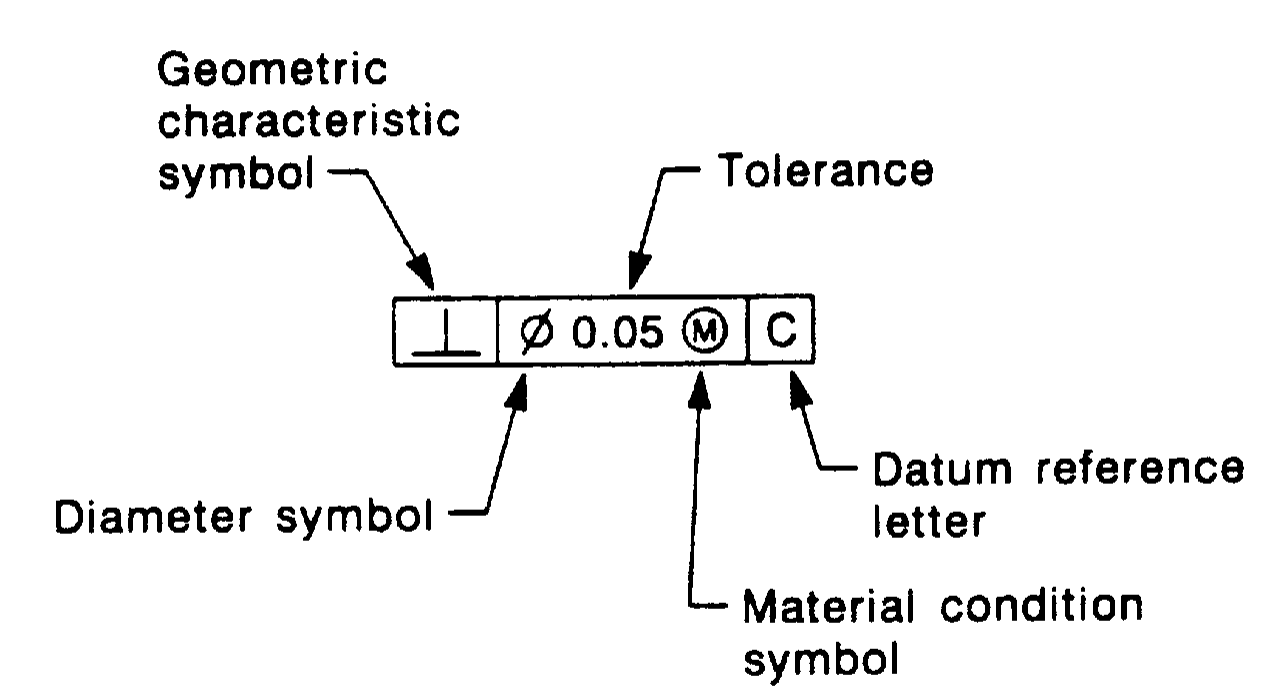
\includegraphics[scale=0.3]{Images/x50_gd&t.png}
\end{center}

where M and L refer to maximum and least material conditions, respectively. Characteristics may be any of the following:

\begin{center}
    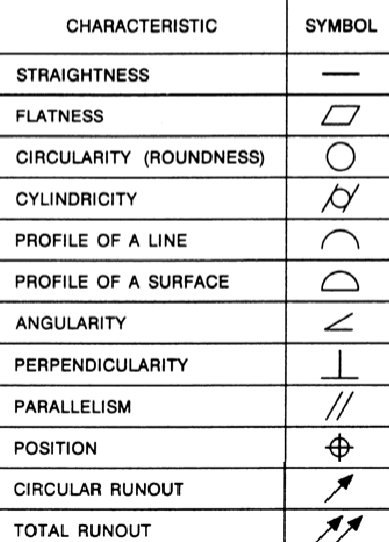
\includegraphics[scale=0.6]{Images/x50_gd&t2.png}
\end{center}

\subsection{Manufacturing Systems}

\textbf{Discrete Manufacturing}

\textit{Discrete manufacturing} refers to the production of distinct items (as opposed to \textit{process manufacturing}, where production is by weight, i.e. chemical or pharmaceutical production). Discrete manufacturing systems can generally be analyzed as a production line, consisting of a series of separate manufacturing stations.

The production rate of an entire line is limited to the production rate of the slowest machine, where the slowest machine is the \textit{bottleneck}. Optimizing the flow rate of a production line therefore involves optimizing the output of the bottleneck. Common ways to improve a process bottleneck include: \begin{enumerate}
    \item Add another bottleneck process in parallel, thus increasing the effective production rate
    \item Place a \textit{buffer} station (accumulating parts from a previous station) before the bottleneck to prevent the bottleneck being \textit{starved}.
\end{enumerate}

Discrete manufacturing occurring over a long period of time may be approximated as a steady-state flow, with constant flow rate $\lambda$ parts per hour. \textbf{Little's Law} simply relates the production rate and the time of production $W$: \[L = \lambda W\] Importantly, Little's Law applies to both a single process and a group of processes (i.e. an entire factory). Therefore, $L$ may be either the number of units in a system or the number of manufacturing stations in a factory, depending on the units of the variable $\lambda$.

\textbf{Takt time} is a measure of the average time between production of units, given by \[\text{takt time} = \frac{\text{production time}}{\text{production quantity}}\] If $1/\lambda > \text{takt time}$, then the production system is too slow and/or the production numbers are unfeasible in the given time.

\textbf{Process Capability}

A \textit{process capability index} is a standard way to measure the variability of a process output within a specification or tolerance. Given an \textit{upper specification limit} USL and a \textit{lower specification limit} LSL, the process capability index $C_p$ is defined by \[C_p = \frac{\text{USL}-\text{LSL}}{6\sigma}\] where $\sigma$ is the standard deviation of measurements on output parts. $C_p$ should ideally be as large as possible, with $C_p>1.33$ being the typical industry-standard minimum. $C_{pk}$ measures both the accuracy and the precision by comparing to the mean value, where $C_{pk}$ is defined by \[C_{pk} = \min \left\{\frac{\text{USL}-\mu}{3\sigma},\frac{\mu-\text{LSL}}{3\sigma}\right\}\] $C_{pk}$ is generally smaller than (or sometimes equal to) $C_p$ and should also be maximized.

\textbf{Manufacturing Cost Modeling}

Total costs involved in the production of $n$ parts of mass $m$ are given by \[C_\text{total} = C_\text{material} + C_\text{capital} + C_\text{energy} + C_\text{overhead}\] Many processes are only viable given large batch size, effectively reducing per-part capital costs.

Whether an investment is likely to be profitable is determined by the related quantities \textit{net present value} (NPV) and \textit{internal rate of return} (IRR). Given an initial investment $C_\text{init}$, cash flow $C_t$ in year $t$, and discount rate (annual return that could be earned with a similar investment, typically between 5\% and 15\%) $i$, the net present value of an investment is computed as \[\text{NPV} = \sum_{t=1}^T\underbrace{\left(\frac{C_t}{(1+i)^t}\right)}_\text{Yearly NPV} - \underbrace{C_\text{init}}\] Similarly, the internal rate of return is the value for which $\text{NPV}=0$, or the solution to \[\sum_{t=0}^T \left(\frac{C_t}{(1+\text{IRR})^t}\right) - C_\text{init} = 0\] If $\text{IRR}<i$, an investment is a bad investment as it does not meet the minimum rate of return a firm could achieve with a similar investment. A higher IRR indicates a more desirable investment, and the best investment among a series of options is that with the highest IRR.

\subsection{Manufacturing Processes}

Manufacturing most fundamentally involves bringing stock material to a desired shape. Each manufacturing process has specific capabilities and associated processing times, making a process more or less feasible depending on the material properties, desired geometry, and the scale of production. 

\textbf{Subtractive Processes}

Subtractive processes involve removing material from a stock piece. Common examples include:
\begin{enumerate}
    \item[] \textbf{Blanking}, a process by which sheet-metal components are produced by shearing. This process is suitable for mass production because of its low processing time and the recyclability of leftover material "skeleton".
    \item[] \textbf{Machining}, where the five basic machining processes are \textit{turning} (on a lathe), \textit{drilling}, \textit{milling}, \textit{grinding}, and \textit{sawing}.
    \item[] \textbf{CNC Processes}, including water jetting, laser cutting, CNC milling, CNC lathing, and other automated processes. CNC machines are programmed with G-Code and generally allow more complex geometries to be produced (in particular with CNC mills and CNC lathes).
\end{enumerate}
Machining processes are relatively slow compared to other methods, and are therefore not suitable for mass manufacturing (i.e. $>$100,000 parts). As an example, for a lathe operation with feed rate $f$ inches/rev, spindle speed $N$ revs/min, initial diameter $D_0$ and a depth of removal $d$, the material removal rate is given by \[\text{material removal rate} = \underbrace{\pi D_0 N}_{v} d f\] where $v$ is the \textit{cutting speed}, the tangential speed of the workpiece. The machining time is then given by \[T_m = \frac{L}{Nf}\]

\textbf{Metal Forming}

Because machining is relatively slow, parts are generally brought near their final shape so that machining becomes a finishing process, rather than a shaping process. The processes here are \textit{bulk deformation processes}, which plastically deform a material, causing \textit{work hardening} and producing a tougher final part: \begin{enumerate}
    \item[] \textbf{Extrusion}. Involves forcing a metal through a die to form a long shape. Metals may be extruded \textit{hot} (aluminum, copper, magnesium) or \textit{cold} (aluminum or steel, with steel requiring high forces).
    \item[] \textbf{Forging}. Produces a part near net shape of very high strength. Types include \textit{open die forging} (suitable for large parts, generally requiring lots of machining) and \textit{closed die forging} (suitable for producing smaller parts near net shape, where only the excess "flash" which squeezes out of the mold must be machined away).
\end{enumerate}

The forces involved in forging can be quite large. The required forces can be evaluated by considering first the necessary deformation, then the strain in the material, then the stress in the material, and finally the surface area of the part.

Strain of work is given by \[\epsilon = \ln \frac{h_0}{h}\] where $h_0$ is the initial height of the stock and $h$ is the final height. The stress is then given by \[Y_f = K\epsilon ^n\] where $K$ is the strength coefficient and $n$ is the strain hardening exponent, both of which are material properties. Finally, the compressive force is found by \[F = K_f Y_f A\] where \[K_f = 1 + \frac{.4\mu D}{h} \text{ (shape factor)}\] $K_f$ is a function of part height and diameter, and also friction between the part and the die. Shape factor $K_f$ is not related the strength coefficient $K$.

There are different metal forming operations available for forming sheet metal parts: \begin{enumerate}
    \item[] \textbf{Simple Bending}. Involves bending straight lines into a sheet metal part using a punch and die. Both cheaper and slower than stamping operations.
    \item[] \textbf{Sheet Metal Stamping}. Involves pressing a sheet metal part between a die and a punch to form a desired shape. Often used in mass production because the process is relatively fast and maintains sheet thickness.
    \item[] \textbf{Sheet Metal Drawing}. Essentially the same as stamping, but with a specialized (more expensive) die allowing part to be drawn to a depth larger than the punch diameter.
\end{enumerate}

\textbf{Additive Manufacturing}

Additive manufacturing processes are varied and involve forming a part from feedstock, rather than forming or removing from existing stock. There are seven categories of additive manufacturing process:

\begin{center}
    \begin{tabular}{ | m{2in} | m{2in} | m{2in} | }
    \hline
    Process & Material Used & Tool Used\\
    \hline
    Material Jetting & Melted Plastic & Laser or Multi-Nozzle Print Head\\
    \hline
    Vat Photopolymerization / Stereolithography (SLA) & Melted Plastic & Laser\\
    \hline
    Material Extrusion & Melted Plastic & Single-Nozzle Print Head\\
    \hline
    Sheet Lamination & Material Sheets & Solid-State Welding or Adhesive\\
    \hline
    Directed Energy Deposition & Powdered Metal & Laser \\
    \hline
    Powder Bed Fusion & Plastic Powder (SLS) or Metal Powder (SLM/DMLS) & Laser\\
    \hline
    Binder Jetting & Powdered Metal & Multi-Nozzle Print Head, then Solid State Welding\\
    \hline
    \end{tabular}
\end{center}

\textbf{Liquid to Shape}.

As opposed to other metal forming processes, metals can also be \textit{cast} into a nearly complete shape. This is accomplished by pouring a molten metal into some form of mold; the hardened metal then takes the desired shape. This process generally requires some amount of machining to process the part, particularly for threads and smooth surfaces, both of which casting is incapable of producing. There are two types of casting: \begin{enumerate}
    \item[] \textbf{Die Casting}. Metal is forced into a permanent die cavity under pressure. Allows for high production rate (suitable for mass manufacturing) and good tolerances and surface finish. Can occur in a \textit{hot chamber} (where low melting point metals, i.e. zinc or magnesium, are under high pressure until they solidify in the mold) or in a \textit{cold chamber} (where metal is melted in a separate furnace and driven into the die). 
    \item[] \textbf{Sand Casting}. Most common casting process, involving a mold made of sand which is broken after the part solidifies. Produces a rough surface finish and has low upfront cost, but is also a slower process as molds are not reused.
\end{enumerate}

A mold used in sand casting consists of a \textit{cope} (top half) and \textit{drag} (bottom half), and often a \textit{core} which produces the internal surfaces on a cast part. The core is supported by \textit{chaplets} both above and below, which are placed below to support the core weight and above to counteract bouyant forces from the molten metal. For core of density $\rho_c$ and volume $V_c$ and molten metal of density $\rho_m$, the forces acting on the core are \[\underbrace{F_b = (\rho_m - \rho_c)V_cg}_\text{bouyant force},\hspace{0.5in}\underbrace{W=\rho_cV_cg}_\text{weight}\] If a chaplet is able to support $F_\text{chap}$, then the number of chaplets necessary is given by \[N_\text{above} = \left\lceil\frac{F_b}{F_\text{chap}}\right\rceil\] Then, enough chaplets must be placed below to support the weight of both the core and the chaplets above. Thus, the number of chaplets required below is \[N_\text{below} = \left\lceil\frac{W +N_\text{above}\cdot W_\text{chap}}{F_\text{chap}}\right\rceil\]

\newpage

Even more diverse processes exist for forming liquid plastic:
\begin{enumerate}
    \item[] \textbf{Injection Molding}. Produces open shapes by forcing high-pressure liquid plastic into a closed mold. Plastic is subject to shrinkage as it cools.
    \item[] \textbf{Blow Molding}. Produces thin, bottle-like shapes with small openings by "blowing" heated plastic to walls of a closed mold.
    \item[] \textbf{Rotational Molding}. Produces thin-walled, seamless, hollow shapes by rotating a mold, forcing liquid plastic to conform to the mold shape.
    \item[] \textbf{Thermoforming}. Produces flat, thin-walled shapes by "sucking" heated plastic sheet onto an open mold.
\end{enumerate}

Parts created in injection molding are particularly vulnerable to shrinkage as they cool within the mold. If a cavity has dimension $D_c$ and a plastic has a shrinkage value $S$ (typically in mm/mm or inch/inch, i.e. unitless), then the dimension of the molded part is given by \[D_c = \frac{D_p}{1-S}\]

\end{document}
